\documentclass[11pt]{report}
\usepackage[brazil]{babel}
\usepackage[utf8]{inputenc}
\usepackage[usenames,dvipsnames,svgnames,table]{xcolor}
\usepackage[a4paper,margin={1in}]{geometry}
\usepackage{color}
\usepackage{textcomp}
\usepackage[bottom]{footmisc}
\usepackage{fancyhdr}
\usepackage{moreverb}
\usepackage{enumitem}
\usepackage{mathtools}
\usepackage[table]{xcolor}
\usepackage{caption}
\usepackage{titlesec}
\usepackage{color,soul}
\usepackage{varwidth}
\usepackage{courier}
\usepackage{tikz}
\usepackage{diagbox}
\usepackage{array}

\newcommand{\quotes}[1]{``#1''}

\titleformat{\section}{\normalfont\Large\bfseries}{\thesection}{1em}{}[{\titlerule[0.4pt]}]

\definecolor{fill}{rgb}{0.18, 0.31, 0.31}
\definecolor{strong}{rgb}{0.5, 1.0, 0.0}
\definecolor{moderate}{rgb}{0.24, 0.82, 0.44}
\definecolor{weak}{rgb}{0.99, 0.05, 0.21}
\definecolor{train}{rgb}{0.59, 0.0, 0.09}
\definecolor{test}{rgb}{0.98, 0.93, 0.36}

\pagestyle{fancy}
\renewcommand{\chaptermark}[1]{\markboth{#1}{}}
\fancyhf{}
\fancyhead[RE]{\chaptername~\thechapter}
\fancyhead[LO]{\leftmark}
\rhead{\chaptername \enspace \thechapter}
\cfoot{\thepage}

\setcounter{secnumdepth}{3}

\newcolumntype{P}[1]{>{\centering\arraybackslash}p{#1}}

\begin{document}

\begin{center}
  \thispagestyle{empty}
  {\LARGE \textbf{Universidade de São Paulo}}
  \vspace*{10px}

  {\LARGE \textbf{Instituto de Matemática e Estatística (IME-USP)}}
  \vspace*{150px}

  {\Large \textbf{Reconhecimento de Entidades Mencionadas em Notificações de Atos de Concentração Econômica do Conselho Administrativo de Defesa Econômica}}
  \vspace*{100px}

  {\Large Aluno: Renan Fichberg}

  \vspace*{1px}
  {\Large Orientador: Prof. Dr. Marcelo Finger}

  \vspace*{150px}
  {\large Monografia de Conclusão de Curso realizado para a disciplina}

  \vspace*{1px}
  {\large MAC0499 - Trabalho de Formatura Supervisionado}

  \vspace*{100px}
  {\large São Paulo, novembro de 2016}
\end{center}

\pagebreak
\thispagestyle{empty}
\chapter*{Agradecimentos}
\markboth{UNNUMBERED CHAPTER}{}

\indent\indent Este trabalho, apesar de ter apenas um autor, possui muito das experiências e conhecimento que acumulei ao longo
do curso de Bacharelado em Ciência da Computação e, reconheço, não seria possível realizá-lo não fosse o aprendizado e o incentivo que tive, de várias
pessoas com quem convivi não apenas na universidade, mas fora dela também. Destaco, a seguir, algumas pessoas com quem tive a chance de aprender
bastante para chegar até o presente momento:

Primeiramente, aos meus pais Eloy Fichberg e Regina Célia de Oliveira Pinto e aos meus irmãos Felipe Fichberg e Leone Fichberg, que sempre foram
as pessoas mais presentes na minha vida, me incentivando a seguir adiante em todos os momentos.

Em seguida, aos meus grandes amigos que acompanharam a minha trajetória de perto, Eduardo Gromatzky Feder e Gabriel Engel Pesso, que sempre foram companheiros
em todos os momentos.

Aos meus colegas e amigos do BCC, Maurício Cardoso, Luiz da Silva Armesto, Renato Cordeiro Ferreira, Pedro de Carvalho Rogrigues, João Marco Maciel da Silva,
Gervásio Santos, Renato Massao, Yara Grassi Gouffon, Rafael Raposa, Lucas Hiroshi Hayashida, Victor Sanches Portella, Luciana Abud, Karina Suemi Awoki, Vinícius Vendramini, Ruan Costa,
Vinícius Bitencourt Matos e tantos outros que percorreram juntos comigo essa trilha e sempre se mostraram dispostos a ajudar.

Aos meus colegas e amigos do Mezuro e do BCC, Rafael Reggiani Manzo, Diego Araújo Martinez Camarinha, Fellipe Souto Sampaio, Heitor Reis Ribeiro, Guilherme Rojas, Alessandro Palmeira e
Daniel Paulino Alves, que sempre tinham algo de novo a ensinar.

Aos meus grandes amigos do colégio, Jonathan Schiriak, Allon Rozansky, Aaron Zarenczanski e Walter Caspari, pelos bons momentos, eventuais apoios e conselhos.

Aos colaboradores deste trabalho, William Collen, Kemil Raje Jarude e o meu orientador Prof. Dr. Marcelo Finger, por toda a paciência que tiveram com as minhas tantas dúvidas e
sugestões de estratégias e ferramentas para solucionar os problemas que foram surgindo.

E finalmente, a todos os professores que tive a oportunidade de conhecer e aprender algo. Todos foram essenciais para a minha trajetória.

\pagebreak
\thispagestyle{empty}
\chapter*{}
\markboth{UNNUMBERED CHAPTER}{}

\vspace*{\fill}
\textit{\quotes{The voice that navigated was definitely that of a machine, and yet you could tell that the machine was a woman, which hurt my mind a little. How can machines have genders? The machine also had an American accent. How can machines have nationalities? This can't be a good idea, making machines talk like real people, can it? Giving machines humanoid identities?}}
\begin{flushright} - Matthew Quick, The Good Luck of Right Now \end{flushright}
\vspace*{\fill}

\pagebreak
\thispagestyle{empty}
\chapter*{Resumo}
\markboth{UNNUMBERED CHAPTER}{}

\indent\indent O Conselho Administrativo de Defesa Econômica (CADE) é um orgão independente que reporta ao Ministério da Justiça e possui como missão garantir a livre
concorrência de mercado em todo o território Brasileiro e realiza as suas funções legais de acordo com a Lei Nº 12.529/2011 [1].
O CADE dispõem de uma base de dados bastante extensa, com processos judiciais de vários tipos distintos datados do ano de 1980 até os dias atuais e mais de 100 tipos diferentes de
documentos, desde formulários, notificações de processos e cópias escaneadas de documentos diversos até arquivos de áudio e vídeo.

A atividade foi dividida em duas partes distintas: a primeira explora parte dos vários processos judiciais presentes na base de dados pública do CADE relacionados a Atos de
Concentração com finalísticos Sumário ou Ordinário e montar um córpus com os tipos de documentos que foram julgados pertinentes em primeira análise. Em seguida, a partir de anotações
manuais de entidades mencionadas e seus relacionamentos sobre o córpus construído, identificar automaticamente as entidades nos processos judiciais futuros que possam ser relevantes a classificação
final entre os dois tipos de rito: Sumário ou Ordinário. A segunda parte, por sua vez, constitui-se da classificação do processo judicial em um dos ritos mencionados por meio de
algoritmos de Aprendizado de Máquina, considerando as entidades que foram encontradas de forma automatizada nos documentos do processo em questão.

Este trabalho trata especificamente da primeira parte e serão aqui abordados assuntos relacionados a ela, tais como Processamento de Linguagem Natural, Reconhecimento de Entidades
Mencionadas e algumas ferramentas de \textit{software} que foram usadas para solucionar o problema em questão. A segunda parte não foi desenvolvida por falta de tempo, infelizmente.

Por fim, além destes conteúdos, também serão compartilhados experimentos e resultados obtidos por meio de validação cruzada com o córpus desenvolvido, junto de possíveis estratégias que
foram aprendidas ao longo do trabalho que poderiam, talvez, melhorar a precisão e a corretude das anotações.

\pagebreak
\thispagestyle{empty}
\chapter*{Abstract}
\markboth{UNNUMBERED CHAPTER}{}

\indent\indent The Administrative Council for Economic Defense (CADE) is an independent agency reporting to the Ministry of Justice and has as mission to ensure to the maximum the free
market competition over the entirety of the Brazilian territory and performs its legal functions according to the Law Nº 12.529/2011 [1].
The CADE owns an extense enough database, with judicial processes of many distinct types dated from the year of 1980 to the present days and over 100 types of different documents,
from formularies, process notifications and scanned copies of diverse documents to audio and video files.

The work was divided in two distinct parts: the first one constituted of exploring part of the many judicial processes within the public database owned by CADE related to Concentrations
Acts with final procedure being either \quotes{Sumário} or \quotes{Ordinário} and build a Corpus with the document types that were considered pertinent in first analysis. After that,
considering manual annotations of named entities and its relationships done over the built Corpus, identify automatically the entities in the future judicial processes that can be relevant
to the final classification between the two types of rite: \quotes{Sumário} or \quotes{Ordinário}. The second part constitutes of the classification of the judicial process in one of
the mentioned rites through the use of Machine Learning algorithms, considering the entities that were found automatically in the documents of the given process.

This work covers specifically the first part and will be discussed here subjects related to it, like Natural Language Processing, Named Entity Recognition and some of software tools that
were used to solve the introduced problem. The second part was not developed duo to the lack of time, unfortunately.

At last, in addition to these contents, experiments and results obtained through the use of cross validation with the created Corpus will also be shared, along with possible strategies that
were learned throughout this project that could, maybe, increase the precision and correctness of the annotations.

\pagebreak
\thispagestyle{empty}
\chapter*{Glossário de Siglas}
\markboth{UNNUMBERED CHAPTER}{}

\indent\indent As siglas descritas a seguir aparecem em partes diversas desta monografia. Confira abaixo
os seus significados:

\vspace*{20px}

\noindent AC - Ato de Concentração

\vspace*{8px}
\noindent AM - Aprendizado de Máquina

\vspace*{8px}
\noindent CADE - Conselho Administrativo de Defesa Econômica

\vspace*{8px}
\noindent DOU - Diário Oficial da União

\vspace*{8px}
\noindent EM - Entidade Mencionada

\vspace*{8px}
\noindent PLN - Processamento de Linguagem Natural

\vspace*{8px}
\noindent REM - Reconhecimento de Entidades Mencionadas

\vspace*{8px}
\noindent RI - Recuperação de Informações

\pagebreak
\thispagestyle{empty}

\tableofcontents

\vspace*{10px}

\hspace*{-0.7cm}
\textbf{Referências}\thinspace\enspace.\enspace.\enspace.\enspace.\enspace.\enspace.\enspace.\enspace.\enspace.\enspace.\enspace.\enspace.\enspace.\enspace.\enspace.\enspace.\enspace.\enspace.\enspace.\enspace.\enspace.\enspace.\enspace.\enspace.\enspace.\enspace.\enspace.\enspace.\enspace.\enspace.\enspace.\enspace.\enspace.\enspace.\enspace.\enspace.\enspace.\enspace.\enspace.\enspace.\enspace.\enspace.\enspace.\thinspace\thinspace\enspace\textbf{47}

\pagebreak
\chapter{Introdução}
\indent\indent Neste primeiro capítulo serão abordados a motivação para o desenvolvimento deste trabalho bem como os seus objetivos e o problema envolvido.
Todo e qualquer conteúdo técnico mencionado aqui será melhor explorado nos capítulos sucessivos, desde assuntos relacionados a áreas da computação, tais como
Reconhecimento de Entidades Mencionadas, até o funcionamento do Conselho Administrativo de Defesa Econômica (CADE), seus processos e a sua base de dados. Assim sendo, o
leitor não deve se preocupar com eventuais dúvidas técnicas que possam surgir com a leitura deste capítulo meramente introdutório.

\section{Motivação}
\indent\indent O tema do projeto é atraente uma vez que está diretamente ligado à realidade da nossa sociedade. O CADE tem um papel
fundamental para manter a concorrência de mercado entre competidores de todos os portes, atuando como um orgão regulador legal. Sua existência é
particularmente importante para dar garantia aos pequenos negócios de não serem engolidos por \textit{players} veteranos, que
já atuam em determinado mercado há mais tempo e, portanto, já dominam fatias consideráveis do público de interesse.

É conhecido também o fato de que os processos judiciais tendem a ser demorados e mesmo que os Atos de Concentração tratados pelo CADE, objetos de estudo deste
trabalho, sejam mais rápidos quando comparados a outros de diferente natureza, tentar torná-los ainda mais rápidos definitivamente é algo benvindo, uma vez que
tais processos judiciais podem demorar até seis meses para terem um tipo de rito escolhido.

A idéia, portanto, é justamente buscar formas de automatizar os processos em andamento de tal forma que exista um ganho tanto para o CADE quanto para a sociedade.
Se tais processos pudessem ser acelerados, em sua totalidade ou partes do \textit{pipeline} envolvido na análise, futuramente a mesma solução poderia ser replicada
para resolver problemas similares com outros tipos de processos judiciais ou mesmo em outras áreas do conhecimento.

\subsection{Retorno}

\indent\indent Para o CADE, isso representaria a possibilidade de resolver mais processos em um mesmo intervalo de tempo, e para organizações ou mesmo cidadãos isso representaria
terem uma resposta mais rápida para planejarem as suas próximas ações. Em especial, é importante ressaltar que estamos lidando com o mercado, que é uma
entidade abstrata muito volátil, isto é: os mercados, de um modo geral, são flutuantes, de tal forma que a sua capacidade de se transformar é altíssima.
Um dado mercado pode estar em alta em um mês e em queda no mês seguinte. Devido em grande parte a globalização, mercados constituem entidades de difícil previsão
mesmo para \textit{experts} em economia.

À luz do que foi dito, portanto, quanto mais próximo da configuração do mercado no momento da petição uma resposta for obtida, melhor será.

\section{Problema}

\indent\indent Dado um conjunto de processos judiciais com ritos conhecidos, queremos buscar saber em quais ritos os processos futuros se encaixarão. Temos dois tipos de classes possíveis para os ritos:
Ordinário e Sumário. Desta forma, este é claramente um problema de classificação binária e já existem maneiras conhecidas de resolvê-lo eficientemente a partir
de técnicas e algoritmos clássicos de AM.

Para conseguirmos desempenhar esta função, porém, é necessário estudarmos as especificidades do problema proposto e, em particular e principalmente,
do tipo de dados com que estamos lidando. Informações com relações a isso serão tratadas no Capítulo 2, Seção 2.2.
Note que esta etapa é essencial para garantirmos não apenas uma maior eficiência na classificação final, mas também que o algoritmo está sendo treinado sobre
documentos totalmente fiéis à realidade.

Acerca do então exposto, surge naturalmente um segundo problema do qual o nosso \textit{approach} por AM irá depender diretamente: construir um córpus para servir de modelo de
treinamento para identificar entidades chaves que podem ser determinantes no julgamento da classe do rito de um futuro processo. Um córpus é, como o próprio nome em latim sugere, um corpo composto de textos.

Assim, uma das possibilidades que surge é usar REM para identificar tais entidades e, a partir destas, buscar alguma relação entre as entidades encontradas e um dos tipos de rito, com
base nos padrões que foram aprendidos a partir do córpus de treinamento criado com processos antigos, presentes na base de dados pública do CADE. Focamos
a nossa atenção, portanto, em primeiramente resolver o problema da construção do córpus para treinamento.

\section{Objetivos}

\indent\indent O principal objetivo deste trabalho foi estudar os Atos de Concentração analisados pelo CADE para poder então, criar um córpus de treinamento e a partir deste classificar
o AC em um dos ritos.

Houve também um estudo do próprio funcionamento do CADE para entender mais sobre o problema e, em particular, um estudo voltado para a sua coletânea de processos
armazenada na sua extensa base de dados pública com o intuito de identificar os tipos de documentos que poderiam ser mais pertinentes à análise dos processos no que diz respeito
à classificação final do rito e também à forma que tais processos deveriam ser tratados para que fossem extraídas destes informações relevantes. Todo este conteúdo pode ser encontrado no
Capítulo 2 - O Conselho Administrativo de Defesa Econômica.

Como objetivo também existiu a necessidade de estudar assuntos relacionados a AI, tais como Processamento de Linguagem Natural e Reconhecimento de Entidades Mencionadas, que serão abordados nos Capítulos 3 e 4, respectivamente.
Ademais, foram estudadas ferramentas de \textit{software} que trabalham com PLN e REM: Apache OpenNLP e o BRAT. Mais será dito sobre elas no Capítulo 5, em suas
respectivas seções. Nestas seções será apresentado um estudo de como funcionam as implementações usadas destas ferramentas e também como tais ferramentas foram
utilizadas para que os resultados apresentados no Capítulo 6 fossem alcançados.

Finalmente, foi estudado a partir da técnica estatística de validação cruzada o desempenho do córpus criado e os tipos de erros que surgiram no processo de geração automatizada
de anotações de entidades mencionadas a partir do modelo de treinamento do córpus, de tal forma que foram percebidas algumas boas práticas com relação ao uso destas ferramentas
para aumentar a eficácia e a precisão das marcações. Tais percepções serão comentadas, também, no Capítulo 6.

Infelizmente, conforme já mencionado no Resumo, o escopo acabou revelando-se grande demais para o tempo disponível, e portanto teve de ser reduzido
ao primeiro problema. Dificuldades encontradas seguem listadas na Seção 7.1.

\pagebreak
\chapter{O Conselho Administrativo de Defesa Econômica}

\indent\indent Neste capítulo serão abordados assuntos relacionados ao Conselho Administrativo de Defesa Econômica, aos Atos de Concentração que devem ser legalmente submetidos a ele e à base de dados pública que ele possui e
que contém tais processos judiciais. Sobre o CADE, será exposto um pouco da sua história e da sua função, para em seguida falarmos sobre o que são os ACs que cabem à sua competência
a análise e, finalmente, sobre a base de dados pública que foi usada para obter os Atos de Concentração que compõem o córpus construído, posteriormente usado para treinarmos um modelo
que busca entidades mencionadas de forma automatiza. Mais informações sobre o córpus serão abordadas no Capítulo 3 e as suas entidades mencionadas no Capítulo 4.

\section{Quem é o CADE?}

\indent\indent Para começarmos a entender o CADE, convém que conheçamos um pouco do seu histórico [2]. Criado pela Lei n° 4.137/62 como um orgão do Ministério da Justiça, o CADE hoje é uma autarquia em regime especial com jurisdição em todo o território nacional. Inicialmente,
era da responsabilidade do Conselho a fiscalização da gestão econômica e do regime de contabilidade das empresas, através da Lei n° 8.884/1994, o CADE transformou-se em uma
autarquia vinculada ao Ministério da Justiça.

Tal lei definia as atribuições do CADE e de outros órgãos que formavam juntos com o Conselho Administrativo de Defesa Econômica o Sistema Brasileiro de Defesa da Concorrência e tinham
como missão garantir a política de defesa da livre concorrência em todo o território nacional. O CADE, em particular, era responsável pelo julgamento dos processos administrativos
que tinham relação com condutas anticompetitivas e também por apreciar Atos de Concentração, tais como aquisições, fusões, \textit{joint ventures} e outros que fossem submetidos
à sua aprovação.

Com a entrada da Lei nº 12.529/2011 em maio de 1012, esta uma nova Lei de Defesa da Concorrência, houve uma reestruturação do Sistema Brasileiro de Defesa da Concorrência e a política
da qual ele era encarregado, de defesa da concorrência, passou por mudanças significativas. Em especial, pela nova legislação, o CADE passou a ser responsável por competências até
então dos outros órgãos do Sistema Brasileiro de Defesa da Concorrência: instruir processos administrativos de apuração de infrações à ordem econômica e também de processos de análise
de Atos de Concentração. Ainda sobre a Lei nº 12.529/2011, a principal mudança introduzida consistia na exigência de submissão
prévia ao CADE de fusões e aquisições de empresas que podem proporcionar efeitos anticompetitivos no mercado, algo que no período anterior a esta Lei poderia ser feito depois destas
operações serem consumadas. Para o CADE, passou a existir então um prazo máximo de duzentos e quarenta dias para análise das operações, prorrogáveis por mais noventa dias
em casos de operações demasiadamente complexas.

Estruturalmente, com a Lei nº 12.529/2011 em vigor, também houveram mudanças: o CADE passou a ser constituído pelo Tribunal Administrativo de Defesa Econômica, pelo Departamento de
Estudos Econômicos e pela Superintendência-Geral. A esta última cabe desempenhar no novo sistema grande parte das funções realizadas outrora pelos órgãos que compunham junto
ao CADE o Sistema Brasileiro de Defesa Econômica antes da entrada da nova Lei de meio de 2012, tais como a investigação e a instrução de processos de repressão ao abuso do poder
econômico e a análise dos atos de concentração.

\section{Atos de Concentração Econômica}

\indent\indent Os Atos de Concentração Econômicas são caracterizados por operações que envolvem duas ou mais empresas independentes, conforme descrito no artigo 90 da Lei 12.529/2011. Tais operações
podem ser aquisições de controle ou incorporações de uma ou mais empresas por outras ou ainda a celebração de contratos associativos, consórcios ou \textit{joint ventures} entre duas
empresas ou mais.

\subsection{Operações}

\indent\indent São as operações, aliadas ao faturamento bruto anual ou volume de negócios no Brasil dos agentes econômicos envolvidos, que caracterizam a necessidade de existência dos
Atos de Concentração [3] analisados pelo CADE. Quando o faturamento bruto anual de uma das empresas envolvidas na operação atinge o patamar mínimo de R\$ 750 milhões e o de uma outra, também envolvida na operação, o patamar de R\$ 75 milhões, o AC deve ser notificado ao CADE.

Considerando esta informação, é particularmente interessante que a aplicação desenvolvida saiba identificar as operações de um dado processo, especialmente
pela razão de que certas operações tendem a seguir mais um ou outro tipo de rito. É relevante ressaltar a observação, no entanto, que o tipo de operação não é uma condição suficiente
para identificar o tipo de rito, mas é um bom indicativo para buscarmos o mais provável. Seguem abaixo
os possíveis tipos de operações que um AC pode ter:

\begin{itemize}
  \item \textbf{Fusão}: são caracterizadas pela união de duas ou mais empresas distintas para formar um novo agente econômico único.
  \item \textbf{Incorporação}: são caracterizadas pelo ato de uma ou mais empresas incorporar total ou parcialmente outras empresas dentro de uma mesma pessoa jurídica,
  de tal forma que o incorporado desaparece como pessoa jurídica, mas o incorporador mantém a sua identidade jurídica após a operação.
  \item \textbf{Aquisição}: são caracterizadas pelo ato de uma empresa adquirir o controle total ou parcial da participação acionária de outra empresa.
  \item \textbf{\textit{Joint venture}}: são caracterizadas pela criação de uma nova empresa a partir da associação entre duas ou mais empresas, de tal forma
  que as empresas que se associaram mantém normalmente suas identidades jurídicas pós operação.
\end{itemize}

\section{Base de Dados Pública}

\indent\indent O CADE possui uma base de dados [4] com processos datados desde 1980 até os dias atuais, de tal forma que
para uma pessoa que não sabe ao certo o que está procurando facilmente pode se perder em meio a tantos tipos de processos. Para nós, porém, eram relevantes apenas
os tipos de processo \quotes{Finalístico: Ato de Concentração Ordinário} e \quotes{Finalístico: Ato de Concentração Sumário}, uma vez que foram os objetos de estudo deste trabalho.

Além dos tipos de processo, há outras informações que podem alimentar o sistema de recuperação de informação para que encontremos o que buscamos, tais como buscar um processo pelo
seu número ou dentro de um determinado período cronológico. Uma vez selecionado um dos tipos de processo que nos é relevante (um dos Atos de Concentração mencionados no parágrafo
anterior), é importante identificarmos os tipos de documentos que nos são relevantes para sabermos onde buscarmos as informações que precisamos.

A lista de tipos de documentos é deveras extensa e para alguém que desconhece o tipo de informação que está contido em cada um destes tipos de documentos, descobrir pode ser uma tarefa
bastante demorada. Precisamos, portanto, de alguma heurística para encontrarmos tipos de documentos que sejam potenciais candidatos a serem considerados de alta relevância para nós.

\subsection{Heurística de Seleção de Tipos de Documentos}

\indent\indent Queremos descobrir, dentre os mais de cem diferentes tipos de documentos presentes na base de dados, aqueles que devem
ter as informações mais pertinentes para nós analisarmos os dados e tentarmos descobrir em qual rito determinado futuro processo será classificado.
Ignorando os tipos de documentos por um instante e acessando os diferentes Atos de Concentração que aparecem em uma pesquisa \quotes{crua} (isto é, com apenas um dos tipos de
processo selecionado), comparando-os um a um, é fácil de identificar que a maioria dos ACs, salve pouquíssimas exceções que provavelmente constituem em processos confidenciais,
possuem os tipos de documentos \quotes{Notificação}, \quotes{Formulário de Notificação} e \quotes{Publicação no DOU}.

Tais tipos de documentos, de acordo com as informações presentes na base de dados, sempre estão entre os primeiros documentos submetidos no instante em que um
Ato é dado como público. Para nós, o instante em que um AC é dado como público tem o mesmo efeito de encará-lo como inicializado, uma vez que não temos qualquer acesso
a documentos confidenciais, e portanto nada podemos inferir sobre eles.
Desta forma, chegamos à seguinte heurística para termos um ponto de partida e selecionarmos os tipos de documentos potencialmente mais interessantes, descrita abaixo:

\begin{enumerate}[label=\textbf{\arabic*.}]
\item Buscamos documentos que frequentemente \quotes{abrem} um Ato de Concentração.
\item Olhamos uma quantidade razoável de processos, digamos 50, e vemos em quantos deles tais documentos estão presentes
\item Supomos que tais documentos não são específicos a um AC e portanto devem ter as informações necessárias para que um novo Ato seja consolidado.
\item Como todo Ato obrigatoriamente segue um dos dois tipos de rito, as informações necessárias devem estar presente nos tipos de documentos selecionados.
\end{enumerate}

O item \textbf{1} da heurística é particularmente importante pois ele encapsula todo o objetivo da nossa aplicação: \textit{não queremos apenas identificar o mais provável tipo de rito
de um determinado Ato de Concentração, mas queremos fazer isso com o mínimo possível de informações}, ou seja: quanto menor for o número de análises necessárias por parte do CADE para 
chegar a uma conclusão relacionada ao rito, melhor.

Esta idéia está diretamente relacionada ao \textit{pipeline} mencionado na Seção 1.1. Suponhamos aqui para ilustrar a idéia do
\textit{pipeline} de análise que um determinado AC pode ter no máximo \textit{n} fases $F_i$ e que $F_1$ e $F_n$ sejam suas fases inicial e final, respectivamente.
Suponhamos ainda que existam vários tipos de documentos $D_j$ que podem fazer parte do AC, mas que certos documentos só podem aparecer em uma fase $F_i$ específica.
Diremos que o valor $V_j$ de um dado documento $D_j$ é tão maior quanto menor for o valor de \textit{i}, para $i = 1, 2, 3 ... n$ e que $V_i \in [0, 1]$ de tal
forma que $V_1 = 1$ é o valor máximo de um documento e $V_n = 0$ o valor mínimo.
Consideremos, finalmente, o AC de \textit{n} = 5 fases composto dos 10 documentos $D_j, 1 \leq j \leq 10$ tais que:

\begin{itemize}
  \item $D_1, D_2, D_3 \in F_1$ documentos que abriram o Ato de Concentração.
  \item $D_4 \in F_2$ documento que foi produzido após análise da fase $F_1$.
  \item $D_5, D_6, D_7 \in F_3$ documentos que foram produzidos após a análise da fase $F_2$.
  \item $D_8 \in F_4$ documento que foi produzido após a análise da fase $F_3$.
  \item $D_9, D_{10} \in F_5$ documentos que foram produzido após a análise da fase $F_4$. Encerramento do Ato de Concentração. Como o rito já foi decidido pelo Conselho,
  não possuem valor para nós.
\end{itemize}

Consequentemente, temos a seguinte relação para os valores de cada um dos \textit{j} documentos considerando o \textit{pipeline} $F_i, 1 \leq i \leq 5$:
\begin{center}
  $1 = V_1 = V_2 = V_3 > V_4 > V_5 = V_6 = V_7 > V_8 > V_9 = V_{10} = 0$
\end{center}

Assim sendo, concluímos que os documentos de maior valor para nós são os mais próximos da fase inicial. Há, porém, uma pergunta que deve ser feita: por qual razão,
necessariamente, deveríamos considerar esta interpretação correta? Está questão já foi respondida: tempo. Existe ainda um outro fator que não foi mencionado aqui e será abordado
na Seção 3.2 - Criação do corpus, que responde a pergunta de outra maneira e portanto complementa a nossa resposta. Para adiantar a idéia, considere que os 3 tipos de
documentos presentes na fase inicial, \quotes{Notificação}, \quotes{Formulário de Notificação} e \quotes{Publicação no DOU} possuem diferentes padrões uma vez que a própria
estrutura dos documentos são diferentes. Para completar o raciocínio, lembre-se: algoritmos de aprendizado de máquina aprendem com base em padrões aprendidos no modelo
de treinamento (ao menos os das ferramentas usadas neste trabalho)!

Abaixo, é exposto um pouco do que cada um destes tipos de documentos contém e a diferença estrutural de cada um deles:

\begin{enumerate}[label=\textbf{\arabic*.}]
\item \textbf{Notificação}: Tem uma estrutura informativa acerca da operação, dos agentes econômicos envolvidos e dos documentos anexos relevantes ao Ato, com pedidos
de acesso restrito para os anexos que contém informações críticas que, na opinião das empresas requerentes, caso os seus concorrentes viessem a conhecer prejudicaria o seu negócio.
\item \textbf{Formulário de Notificação}: Tem uma estrutura de perguntas e respostas, onde os agentes econômicos envolvidos respondem ao formulário do CADE. Nem todas as perguntas
são respondidas, pois mais uma vez, certas respostas as requerentes querem que se mantenham confidenciais.
\item \textbf{Publicação no DOU}: Contém poucas linhas, com informações gerais do Ato tais como as organizações envolvidas, seus advogados, número do processo, operação objeto
e setor econômico envolvido, declarando o AC público.
\end{enumerate}

\section{Ritos de um Ato de Concentração}

\indent\indent Até agora, já foi dito muito sobre o objetivo de classificar os Atos em ritos Sumário ou Ordinário, mas nada foi falado a respeito deles. Esta seção, portanto,
é dedicada a entendermos um pouco sobre eles: o que são e  qual é a sua relevância.

\indent Dizemos que um dado processo segue rito ou procedimento Sumário quando ele é simplificado de forma a ser concluído mais rápido. Tal procedimento pode ser
aplicado pelo CADE aos casos em que for considerado de pouco potencial ofensivo à concorrência as operações suficientemente simples. Percebemos, portanto, que a decisão de enquadramento do pedido de aprovação pelo procedimento Sumário é adotada pelo CADE em casos de conveniência e oportunidade, considerando experiências passadas adquiridas com relação a identificação
dos Atos que sejam potencialmente menos agressivos à concorrência.

Existem algumas características que tendem a ser enquadráveis em procedimento Sumário, descrita na Resolução CADE Nº 2, de 29 de maio de 2012 [6], tais como:

\begin{enumerate}[label=\textbf{\Roman*.}]
\item \textit{Joint ventures} clássicas ou cooperativas, que visa apenas a participação em um mercado cujos produtos e serviços não
estejam horizontal ou verticalmente relacionados.
\item Substituição de agente econômico nos casos em que a empresa adquirente não participava, antes do Ato, do mercado envolvido direta ou indiretamente.
\item For provada baixa participação de mercado com sobreposição horizontal.
\item For provada baixa participação de mercado com integração vertical.
\item Ausência de nexo de causalidade, isto é, concentrações horizontais que resultem em variação do Índice Herfindahl–Hirschman (IHH) inferior a 200 com uma operação que não gere controle de mais da metade do mercado relevante. O IHH [20] é uma medida da dimensão das empresas relativamente à sua indústria. Também serve de indicador do grau de concorrência entre as empresas.
\item Outros casos que forem considerados simples, a critério da Superintendência-Geral.
\end{enumerate}

Em teoria, todo o procedimento é considerado Ordinário até que se prove o contrário. Na prática, porém, o que se encontra é que a maior parte dos procedimentos são Sumários.

Ao submeter um Ato de Concentração à apreciação do CADE, as requerentes devem também submeter as respostas do Formulário de Notificação, que é diferente dependendo do rito.
O procedimento Ordinário possui 12 seções a serem respondidas, enquanto o Sumário possui apenas 7. Ainda, estas 7 seções do procedimento Sumário estão contidas no
procedimento Ordinário, mostrando que, de fato, o que difere um rito do outro é apenas a complexidade.

\pagebreak
\chapter{Processamento de Linguagem Natural}

\indent\indent Neste capítulo falaremos um pouco sobre Processamento de Linguagem Natural (PLN) [7], um campo da Ciência da Computação já bastante maduro que começou a ser muito
explorado a partir do ano de 1950, apesar de ainda antes desta data ser possível encontrarmos trabalhos realizados em PLN. Problemas relacionados a
Processamento de Linguagem Natural envolvem o entendimento de linguagens naturais por parte das máquinas ou mesmo geração de linguagem natural (isto é, a conversão
de uma representação entendida por computadores em uma representação em linguagem natural).

Estamos particularmente interessados na primeira
categoria de problemas de PLN mencionada, uma vez que os Atos de Concentração estão escritos em linguagem natural, mais especificamente o português, e buscamos extrair informações
deles. Isso significa, naturalmente, que é necessário que exista algum entendimento por parte da máquina sobre o conteúdo presente nos ACs, usados para construir nosso córpus. Sendo
assim, nosso ponto de partida neste capítulo será justamente o córpus.

\section{Corpus}

\indent\indent Já falamos muitas vezes a palavra córpus neste trabalho, mas afinal, o que é um córpus? Conforme já mencionado na Seção 1.2, um córpus é um corpo composto de textos. Para trabalhar com um córpus, é necessário que este seja suficientemente extenso.

Mas de quão extenso estamos falando, afinal? Um exemplo de córpus extenso é o Brown University Standard Corpus of Present-Day American English\footnote[1]{
Versões do Brown Corpus podem ser encontradas na internet.} (ou apenas Brown Corpus) [8], compilado na década de 1960 na universidade de Brown, Providence, Rhode Island, como um Corpus de
propósito geral no campo de linguística de corpus. Ele contém 500 exemplares de textos em inglês americano, com cerca de um milhão de palavras. Um córpus mais modesto é o Susanne Corpus [9],
com aproximadamente cento e trinta mil palavras, que é na realidade um subconjunto do Brown Corpus.

De acordo com os autores Christopher D. Manning e Hinrich Schuetze [10], apenas para fazer a ordenação do Brown Corpus e criar uma lista de palavras nos primeiros anos de trabalho na
sua construção eram necessárias 17 horas dedicadas de tempo de processamento, uma vez que os computadores tinham poucos kilobytes de memória. E os problemas não terminavam por aí,
uma vez que para trabalhar com documentos deste tamanho também necessitava de discos rígidos grandes o suficiente para armazená-los. Isso significa que, apesar de PLN ser uma área
que já vem sendo explorada há algum tempo, a tecnologia poderia facilmente ser o gargalo a depender da estratégia que fosse escolhida para buscar a solução do problema. Felizmente,
com simples computadores atuais podemos realizar estas mesmas tarefas em questão de minutos.

Agora que já sabemos de que se trata um córpus, falaremos na seção a seguir sobre o que precisamos ter em mente para criarmos um córpus.

\subsection{Criação do Corpus}

\indent\indent Criação de um córpus é mais complicado do que aparenta, e é um processo que apenas através da experiência empírica podemos ter uma idéia do
quão bom está o córpus que estamos montando. Existem alguns pontos de extrema relevância que devem ser considerados por alguém que está inclinado a submeter-se a esta
tarefa, destacados abaixo:

\begin{enumerate}[label=\textbf{\arabic*.}]
  \item \textbf{Linguagem}: A linguagem natural em questão. Trabalhar com textos em diferentes línguas pode não trazer bons resultados, uma vez que as línguas possuem regras
  gramaticais diferentes e diferentes formas de construção de sentenças. Frequentemente uma pessoa que está montando um córpus irá querer submetê-lo a outros processos diversos
  tais como o de tokenização e o de segmentação de sentenças e estes podem se comportar diferentemente dependendo da linguagem natural em que os documentos estão escritos.
  \item \textbf{Estrutura}: A estrutura do documento, de acordo com o seu tipo, convém ser similar para todos os documentos envolvidos na montagem do Corpus. Não convém
  misturar em um mesmo córpus, por exemplo, documentos com um formato de perguntas e respostas, tais como um formulário, com um outro documento que segue um formato dissertativo.
  A depender dos tipos de documentos que estão sendo misturados, isso pode mais atrapalhar do que ajudar na hora de buscar extrair certas informações, uma vez que os padrões
  no texto que estão sendo submetidos ao algoritmo de aprendizado podem ser muito diferentes. Pode ser que ao fazer isso, estejamos introduzindo \quotes{confusão} ao processo
  de aprendizado de máquina.
  \item \textbf{Representatividade}: Conforme mencionado por Christopher D. Manning e Hinrich Schuetze [10], os textos que formam o córpus precisam constituir uma amostra
  representativa da população de interesse. Em outras palavras, um determinado córpus precisa ser fiel aos documentos reais. Para o caso deste trabalho, este item é o principal
  motivador para que construíssemos um córpus considerando os Atos de Concentração passados na base de dados pública do CADE ao invés de usar qualquer outro córpus de propósito
  geral para a língua portuguesa, tal como o Córpus Amazônia [11], disponibilizado pelo sítio da linguateca [13].
  \item \textbf{Tamanho}: O tamanho do córpus. É de se esperar que um córpus maior tenha mais exemplos para que o algoritmo possa gerar algum aprendizado, portanto, córpus grandes 
  e coerentes com os três itens apresentados anteriormente devem conseguir atingir resultados mais satisfatórios.
\end{enumerate}

O córpus desenvolvido neste trabalho foi criado a partir de cinquenta Atos de Concentração Econômica. O critério de escolha de tais atos foi utilizar os mais recentes, assim,
todos os processos utilizados não necessariamente começaram no ano de 2016, mas estavam ou estão abertos ainda neste ano. A razão de escolher os mais recentes é para dar um pouco
mais de garantia que nosso córpus é um pouco mais fiel à realidade, apesar dos ACs mais antigos aparentarem seguir a mesma forma de apresentação das informações.

Ainda, destes cinquenta processos, uma metade é composta de procedimentos Sumários e a outra de procedimentos Ordinários, de tal forma que obtivéssemos um córpus resultante balanceado
com relação à representação dos ritos. Mesmo sabendo que na prática há muitos mais ritos Sumários que Ordinários, para efeitos de aprender a classificar, foi julgado mais
interessante que as amostras de cada um dos tipos aparecessem nas mesmas proporções. Na tabela 3.1 a seguir, são listados os números dos processos utilizados:

  \begin{table}[h!]
    \centering
    \begin{tabular}{| c | c | c | c |}
      \hline
      \multicolumn{4}{|c|}{Nº dos Processos} \\
      \hline
      \multicolumn{2}{| c }{Ordinários} & \multicolumn{2}{| c |}{Sumários} \\
      \hline
      08700.000722/2016-54 & 08700.004168/2016-84 & 08700.000625/2016-61 & 08700.005269/2016-72 \\
      08700.000723/2016-07 & 08700.004211/2016-10 & 08700.001192/2016-61 & 08700.005334/2016-60 \\
      08700.001221/2016-95 & 08700.004360/2016-71 & 08700.003684/2016-91 & 08700.005387/2016-81 \\
      08700.001872/2016-85 & 08700.004557/2016-18 & 08700.003951/2016-21 & 08700.005456/2016-56 \\
      08700.002432/2016-45 & 08700.004860/2016-11 & 08700.004768/2016-42 & 08700.005457/2016-09 \\
      08700.002792/2016-47 & 08700.005093/2016-59 & 08700.004963/2016-72 & 08700.005559/2016-16 \\
      08700.003024/2016-19 & 08700.005398/2016-61 & 08700.005000/2016-96 & 08700.005580/2016-11 \\
      08700.003045/2016-26 & 08700.005524/2016-87 & 08700.005002/2016-85 & 08700.005587/2016-33 \\
      08700.003252/2016-81 & 08700.005683/2016-81 & 08700.005138/2016-95 & 08700.005603/2016-98 \\
      08700.003421/2016-82 & 08700.005702/2016-70 & 08700.005139/2016-30 & 08700.005619/2016-09 \\
      08700.003462/2016-79 & 08700.005733/2016-21 & 08700.005204/2016-27 & 08700.005620/2016-25 \\
      08700.003636/2016-01 & 08700.010790/2015-41 & 08700.005208/2016-13 & 08700.005667/2016-99 \\
      08700.003952/2016-75 & \cellcolor{fill} & 08700.005259/2016-37 & \cellcolor{fill} \\
      \hline
      \multicolumn{4}{| c |}{Total: 50} \\
      \hline
    \end{tabular}
  \caption{Número dos processos usados na construção do córpus, todos do ano de 2016.}
  \end{table}

O córpus resultante tem exatamente 50351 palavras\footnote[2]{Resultado obtido através do utilitário \textbf{wc}. Isso significa que, a rigor, o número de palavras
reais é um pouco menor, dado que coisas como numeração de itens são consideradas palavras.}, portanto, é um córpus pequeno. O objetivo inicial era que o córpus
possuisse 300 mil palavras, o que significaria utilizarmos aproximadamente 6 vezes o número de processos utilizados, ou seja, cerca de 150 processos Sumários e
150 processos Ordinários, totalizando mais ou menos 300 processos. A meta, porém, não foi atingida pelas seguintes razões:

\begin{enumerate}[label=\textbf{\arabic*.}]
  \item \textbf{Disponibilidade da Base}: Não foi um problema frequente, mas de vez em quando a base de dados poderia estar fora do ar.
  \item \textbf{CAPTCHA}: A cada busca de documentos que é realizada na base de dados do CADE, o usuário deve submeter uma resposta a um teste CAPTCHA. Isso
  retarda o processo de obtenção de documentos consideravelmente e dificulta bastante para realizar uma tarefa de obter os documentos de forma automatizada, de tal
  forma que era mais simples fazer o processo manualmente.
  \item \textbf{Formato dos Documentos}: Todos os documentos da base de dados do CADE estão em \textit{Portable Document Format} (PDF), que é um formato agradável à
  leitura humana, mas não é dos melhores para leitura de máquina. Houve a necessidade, portanto,  de trabalharmos usando \textbf{Tesseract OCR} para fazer a conversão do
  formato PDF para textos em \textit{American Standard Code for Information Interchange} (ASCII).
  \item \textbf{Qualidade do Escaneamento}: Todos os textos presentes na base de dados são legíveis para humanos, entretanto muito deles estão com uma qualidade ruim para
  o uso do OCR. Alguns documentos tiveram de ser descartados justamente por produzirem uma resposta muito ruim após conversão.
  \item \textbf{\quotes{Sujeira} e Erros de OCR}: Mesmo os documentos que estavam com uma qualidade aceitável produziram \quotes{lixo}, que tiveram de ser descartados
  manualmente. Ainda, foram extremamente comuns erros de substituição de caracteres, em particular os latinos. Trocas de sílabas tais como "ção" e "são" muitas vezes eram
  interpretadas como "gao" ou "cao" e "6ao" e tiveram de ser corrigidas manualmente. Note que usar mecanismos de substituição automática não garantem a correção do problema,
  pois sílabas erradas em um palavra podem ser corretas em outra, portanto, ao tentarmos fazer correção automatizada, apenas transferimos muitas vezes o erro de uma palavra
  para a outra, de tal forma que é necessário passar por um processo de correção humana.
  \item \textbf{Literatura}: Ler e entender textos escritos na linguagem técnica do direito não é algo trivial uma vez que estes textos são bastante densos em informações e
  possuem um vocabulário complicado.
  \item \textbf{Exaustão}: Todos os processos manuais envolvidos unidos à dificuldade da literatura do direito legal inevitavelmente acrescentam \quotes{erros de exaustão}
  por se tratar de um processo cansativo para quem está corrigindo.
  \item \textbf{Tempo Disponível}: O prazo de 1 ano para o desenvolvimento do trabalho impede que o córpus seja muito maior. Este córpus de 50000 palavras tomou pouco menos de 2 meses
  para ser apenas construído e corrigido, sendo que o processo mais demorado é o de anotação, que será mencionado na próxima seção. É relevante considerar que este trabalho
  todo foi feito por apenas uma pessoa.
\end{enumerate}

Na seção a seguir falaremos sobre as anotações.

\subsection{Anotações}

\indent\indent Apesar de não constituir de uma regra, é comum que alguém que esteja trabalhando com um córpus faça diferentes tipos de anotações sobre o mesmo.
Há diferentes tipos de anotações que podem ser feitas, tais como tokenização, detecção de sentenças, etiquetas morfológicas (\textit{part-of-speech tagging}) entre outras, todas
usadas para extrair diferentes tipos de informações dos textos. Em particular, mais será abordado sobre as duas primeiras nas próximas seções.

Anotações, portanto, constituem de metadados sobre os dados. Comumente, linguagens como \textit{Standard Generalized Markup Language} (SGML) ou
\textit{eXtensible Markup Language} (XML) são utilizadas para fazer marcações sobre texto, mas
neste trabalho, as anotações foram feitas utilizando uma ferramenta relativamente nova chamada BRAT, que possui um
formato próprio e que o Apache OpenNLP, uma ferramenta celebrada na área de Processamento de Linguagem Natural, reconhece o formato.
Mais será falado sobre estas ferramentas no Capítulo 5.

\section{Tokenização}

\indent\indent Tokenização é frequentemente um dos primeiros processos envolvidos no processamento de textos escritos em linguagens naturais. Uma \textit{token} nada mais é que uma
palavra, um número ou mesmo pontuações (só que o tratamento de pontuações, especificamente, pode variar de acordo com o texto em questão)[10]. Naturalmente, surge a necessidade de
definir, portanto, o que é uma palavra.

Conforme sugerido em (Kučera e Francis, 1967), uma palavra, para efeitos computacionais, é uma \textit{string} com caracteres alfanuméricos
contíguos, delimitada por espaços em branco e que pode conter hífens e apóstrofos e mais nenhuma outra forma de pontuação. Tal definição é demasiadamente simplista,
mas pode funcionar a depender do tipo de texto que está sendo usado. Uma outra aproximação ainda menos sofisticada é a estratégia do utilitário \textbf{wc}, já mencionado
aqui na nota de rodapé número 8, que simplesmente considera caracteres contíguos delimitados por espaços em branco como uma palavra, independente da sua natureza. Assim, por exemplo,
a \textit{string} de dois caracteres C\# será considerada uma palavra de acordo com a segunda definição, mas não com a primeira.

Fica claro, portanto, que a definição de palavra a ser usada é fundamental para efeitos de marcação e que esta vai afetar diretamente os resultados obtidos, de tal forma que as
respostas conseguidas com um córpus que considera palavras com uma definição A gerará saídas diferentes do mesmo córpus considerando palavras com uma definição B.

\subsection{Tokenização nas Notificações dos Atos de Concentração}

\indent\indent Existem outros problemas que surgem no processo de Tokenização além do que será considerado uma palavra. Um leitor observador pode ter percebido que ambos os exemplos anteriormente
mancionados colocam grande importância nos espaços em branco para delimitar uma palavra, porém existem linguagens naturais que não fazem uso do espaço em branco entre palavras, e
estes problemas também são pertinentes ao processo de Tokenização. Ainda, palavras não aparecem sempre delimitadas entre espaços em branco em um texto. Considere o seguinte trecho,
retirado da Notificação do Ato de Concentração nº 08700.004168/2016-84:

\begin{quote}
  \textit{\quotes{16. Conforme exigido no art. 110, §3 da Resolução CADE nº 1/2012, as Requerentes declaram que (i) todas as informações apresentadas são, ao que é de seu
  conhecimento, verdadeiras e corretas; (ii) todos os documentos e cópias de documentos anexos à presente notificação são autênticos ou cópias fiéis de suas versões originais;
  e (iii) todas as estimativas foram feitas de boa-fé, de acordo com as melhores informações disponíveis.}}
\end{quote}

Vejamos o que acontece com o seguinte trecho considerando as duas aproximações mencionadas anteriormente destacando os problemas encontrados em ambas em \hl{amarelo}.

\textbf{I.} Aproximação de (Kučera e Francis, 1967): caracteres alfanuméricos contíguos, com hífens e apóstrofos, delimitados por espaços em branco constituem uma palavra.

\begin{quote}
  \textit{\quotes{\hl{16}. Conforme exigido no \hl{art}. \hl{110}, §\hl{\mbox{3}} da Resolução CADE \hl{n}º \hl{1/2012}, as Requerentes declaram que \hl{(i)} todas as informações apresentadas \hl{\mbox{são}}, ao que é de seu
  \hl{conhecimento}, verdadeiras e \hl{corretas}; \hl{(ii)} todos os documentos e cópias de documentos anexos à presente notificação são autênticos ou cópias fiéis de suas versões \hl{originais};
  e \hl{(iii)} todas as estimativas foram feitas de \hl{\mbox{boa-fé}}, de acordo com as melhores informações \hl{\mbox{disponíveis}}.}}
\end{quote}
\begin{center}
  Exemplo 3.1: Tokenização pela aproximação dos autores Kučera e Francis.
\end{center}


Com relação a esta aproximação notavelmente há problemas relacionados a \textit{períodos}. Pontuações como vírgula, ponto-e-vírgula e ponto final acabam frequentemente sendo um dos
delimitadores de algumas palavras ao invés de um espaço em branco. Há também pontos em abreviações, como no caso de \quotes{art.}, e o caractere \quotes{/} que faz parte do número da
Resolução do CADE mencionada no trecho. Notemos ainda que o trecho é o décimo sexto item de alguma seção do documento, então o ponto que sucede o 16 configura outro tipo de problema,
aqui também relacionado ao delimitador ser diferente de um espaço em branco. As listagens dos itens em algarismos romanos entre parenteses e o caractere especial \quotes{§} que antecede o número
do artigo também são problemáticos no que diz respeito a esta aproximação. Em todos estes casos, estas palavras \textit{não serão consideradas palavras} pelo processo de tokenização.\pagebreak

\textbf{II.} Aproximação do utilitário \textbf{wc}: caracteres contíguos, delimitados entre espaços.

\begin{quote}
  \textit{\quotes{16. Conforme exigido no art. \hl{110,} §3 da Resolução CADE nº \hl{1/2012,} as Requerentes declaram que (i) todas as informações apresentadas \hl{\mbox{são,}} ao que é de seu
  \hl{conhecimento,} verdadeiras e \hl{corretas;} (ii) todos os documentos e cópias de documentos anexos à presente notificação são autênticos ou cópias fiéis de suas versões \hl{originais;}
  e (iii) todas as estimativas foram feitas de \hl{\mbox{boa-fé,}} de acordo com as melhores informações \hl{\mbox{disponíveis.}}}}
\end{quote}
\begin{center}
  Exemplo 3.2: Tokenização pela aproximação do utilitário wc com parâmetro -w.
\end{center}

Curiosamente, um problema contrário ocorre com a segunda definição. Aqui, conforme pode ser visto acima, as pontuações de período \textit{são consideradas parte das palavras}, algo
indesejado a depender do tipo da aplicação.

Desta forma, fica claro que a depender do resultado que se está procurando, uma tokenização pode obter resultados melhores ou piores que outra.
\textbf{Considerando apenas as duas aproximações apresentadas}, para efeitos deste trabalho,
vale recordar que como estamos lidando com tecnologia de OCR, parece ser mais vantajoso considerar a aproximação do utilitário \textbf{wc} sobre a dos autores
Francis e Kučera, de tal modo que assim diminuiríamos os riscos de descartar palavras relevantes em determinados contextos.

Ainda, além da questão do OCR, sabemos que os Atos de Concentração são constituídos de documentos oficiais de grandes organizações, ora submetidos à apreciação das
autoridades legais do CADE, e portanto não devem apresentar cadeias de caracteres contíguas inesperadas, fora do português (com um ou outro estrangeirismos
potencialmente oriundos do inglês).

Por fim, não é um problema que a pontuação do período seja incluída nas \textit{tokens} para nós, uma vez que ela não é capaz de eliminar sozinha o sentido do contexto da qual
a \textit{token} foi retirada. O modelo de tokenização usado no trabalho é fornecido na página do Apache OpenNLP para a língua portuguesa. Apesar de não ser o ideal, ele se comporta
dentro do esperado. Idealmente, deve-se considerar criar um córpus composto de Atos de Concentração para treinar a tokenização e gerar um modelo com melhor representatividade.

\section{Detecção de Sentenças}

\indent\indent Outro processo que frequentemente aparece nas primeiras etapas junto à tokenização é o de detecção de sentenças. Este processo consiste em
quebrar um texto em sentenças e é importante por uma série de razões, como o uso posterior de \textit{POS Tagging} e, no nosso caso, Reconhecimento de Entidades Mencionadas, uma
vez que estes processos posteriores precisam saber onde começam e terminam uma sentença para buscar as palavras que devem ser etiquetadas. Outros nomes que o processo de
detecção de sentenças possui são Quebra de Sentenças (\textit{Sentence Breaking}) e Desambiguação de Fronteira de Sentença (\textit{Sentence Boundary Disambiguation - SBD}) [12].

Semelhantemente ao processo de tokenização, no qual surgia a necessidade de saber o que é uma palavra, aqui precisamos saber, então, o que é uma sentença. Uma das aproximações
mais comuns é identificar os períodos, pois 90\% deles são indicadores de limites de sentenças (Riley 1989), conforme descrevem Manning e Schuetze [10] em seu livro.

Já havíamos chamado atenção aos períodos na seção anterior, quando falamos de tokenização, e agora em detecção de sentenças eles ressurgem com uma importância ainda maior. Finais de
períodos são frequentemente marcados por pontuações tais como os pontos final, de interrogação, de exclamação dentre outros, mas nem toda linguagem natural faz uso
de pontuações, como por exemplo o tailandês.

Os autores Manning e Schuetze [10] em seu livro mencionam também pesquisas diversas em detecção de sentenças que foram realizadas ao longo das últimas décadas e o quanto
os resultados melhoraram no decorrer deste tempo, de tal forma que hoje em dia já são conhecidas técnicas para predição de identificação das fronteiras de sentenças com uma
taxa de precisão superior a 99\%.

Conforme pode ser observado com o aqui exposto e de acordo com (Indurkhya e Damerau, 2010) [13], o escopo do problema de detecção de setenças varia de acordo com o idioma
a ser trabalhado. Além disso, os autores também consideram a importância do contexto: supondo que tenhamos diferentes córpus, a maneira como os documentos que os
constituem são redigidos variam de acordo com o meio. Por exemplo, um córpus formado apenas de textos jornalísticos pode ter sentenças com padrões diferentes de um outro
córpus formado apenas pelas obras de autoria de William Shakespeare.

\subsection{Detecção de Sentenças nas Notificações dos Atos de Concentração}

\indent\indent Apesar das Notificações dos ACs seguirem um padrão, tais documentos são redigidos por pessoas diferentes, representando diferentes organizações, e inevitavelmente
podem acabar tendo estilos de escrita um tanto diferentes uns dos outros. Estes estilos podem acabar sendo refletidos diretamente no uso das pontuações, e consequentemente,
na identificação das fronteiras de um período, causando flutuações pequenas.

Um problema que surge, em particular, é o de que a depender do tipo de literatura em questão, os períodos tendem a ter um número médio de palavras, enquanto que
nos Atos, certos períodos podem ser demasiadamente compridos, fugindo um pouco das regras e dificultando a tarefa para o modelo de quebra de sentenças.
Por exemplo: todos os Atos de Concentração se iniciam com um pequeno resumo apresentando as organizações envolvidas, o pedido formal de submissão do AC à apreciação do CADE
com referências às Leis e contratos pertinentes à ação, e vez ou outra também o pedido do tipo de rito sumário ou ordinário e a operação que anseiam realizar.

Este pequeno resumo, para efeitos de REM, é especialmente complicado de ser quebrado em sentenças, uma vez que sempre aparecem entidades mencionadas
em uma posição do texto que estão relacionadas a outras entidades em outras posições, consideravelmente distantes. Notemos ainda que estes trechos não possuem interrogações, exclamações ou pontos finais (exceto o último), de tal forma que o pequeno resumo deve ser considerado \textit{inteiro} a própria sentença.

Um exemplo destes resumos presentes nas Notificações dos ACs é reproduzido a seguir, retirado do Ato de Concentração nº 08700.005683/2016-81:

\begin{quote}
  \textit{\quotes{UNIPAR CARBOCLORO S.A. (“Unipar Carbocloro”), sociedade anônima de capital aberto devidamente constituída de acordo com a legislação brasileira, com sede na Rua
  Joaquim Floriano, nº 960, 15º andar, Itaim Bibi, CEP 04534—004, na cidade de São Paulo, no Estado de São Paulo, no Brasil, SOLVAY INDUPA S.A.I.C. (“Solvay Indupa”),
  sociedade anônima de capital aberto devidamente constituída de acordo com a legislação argentina, com sede na Avenida Alicia Moreau de Justo, 1930, 4º andar, na cidade de
  Buenos Aires, na Argentina, e SOLVAY INDUPA DO BRASIL S.A. (“Indupa Brasil” e, em conjunto com a Unipar Carbocloro e com a Solvay Indupa, “Requerentes”), sociedade anônima
  de capital fechado devidamente constituída de acordo com a legislação brasileira, com sede na Rua Urussui, 300, 3º andar, Itaim Bibi, CEP 04542-903, na cidade de São Paulo,
  no Estado de São Paulo, no Brasil, vêm, respeitosamente, por seus advogados, submeter à apreciação do Conselho Administrativo de Defesa Econômica (“CADE”), em observância aos
  artigos 53, 88 e 90 da Lei 12.529, de 30 de novembro de 2011, a aquisição do controle societário da Solvay Indupa pela Unipar Carbocloro.}}
\end{quote}

Conforme podemos ver no exemplo acima, de fato, a única pontuação que pode ser considerada tradicionalmente como o final de uma sentença só ocorre com o término do trecho. Este trecho
sozinho tem exatamente \textit{181 palavras}, considerando a aproximação do \textbf{wc}, que é um número \textbf{muito distante} do que um \quotes{período normal} contém. A média
de caracteres considerando os resumos de todos os processos que constituem o nosso córpus, listados na tabela 3.1, é de \textit{140.72 palavras por resumo}.

Uma observação final: apesar do exemplo acima conter quase 40 palavras a mais que a média calculada, este não é o resumo que contém mais palavras.

É importante ressaltar aqui que, assim como no processo de tokenização, foi usado o modelo de detecção de sentenças fornecido na própria página do Apache OpenNLP, uma vez que o tempo era
apertado para desenvolver um córpus para servir de treinamento para quebra de sentenças. Os resultados, apesar de serem satisfatórios, poderiam ser refinados com um modelo
de detecção de sentenças criado a partir de Atos de Concentração, uma vez que, assim como na tokenização, aumentaríamos a representatividade do córpus com relação aos documentos
reais.

No próximo capítulo discutiremos sobre REM e como foram feitas as marcações no córpus. Até este ponto, tudo o que foi discutido no Capítulo 2 e neste Capítulo 3 são
requisitos para poder trabalhar com REM nos Atos de Concentração, e uma vez entendidos, será mais simples para o leitor entender a forma que o Reconhecimento de Entidades
Mencionadas foi usado para chegarmos aos resultados e conclusões apresentados nos dois capítulos finais desta monografia.

\pagebreak
\chapter{Reconhecimento de Entidades Mencionadas}

\indent\indent Neste capítulo falaremos um pouco sobre Reconhecimento de Entidades Mencionadas (REM) [16], uma subtarefa da área de Extração de Informações que busca localizar e classificar
palavras de um texto escrito em alguma linguagem natural em entidades previamente definidas tais como nomes de pessoas e nomes de organizações. Também mostraremos como
aplicamos o Reconhecimento de Entidades Mencionadas para os Atos de Concetração Econômica que são apreciados pelo Conselho Administrativo de Defesa Econômica.

\section{Entidades Mencionadas}

\indent\indent Não faz sentido falarmos sobre Reconhecimento de Entidades Mencionadas sem saber, de certo, o que é uma entidade mencionada (ou entidade nomeada), portanto este
será o nosso ponto de partida neste capítulo. Afinal, do que se trata uma entidade mencionada?

Uma entidade mencionada é um objeto que existe no mundo real e que possui um nome próprio [15], como por exemplo, uma pessoa ou uma organização, tal como já foi mencionado na introdução
deste capítulo. Note, porém, que pessoas e organizações possuem naturezes existenciais diferentes, no sentido de que uma pessoa pode ser encarada como um objeto \textit{físico} do mundo real
ao passo que uma organização pode ser encarada como um objeto \textit{abstrato}. Independente disso, porém, ambas possuem seus \textit{tipos de entidade} muito bem definidos
(pessoa e organização) e para efeitos de entidades mencionadas, não é relevante que determinado objeto seja necessariamente real ou virtual.

É relevante ressaltar que entidades mencionadas são temporais no sentido de que certos tipos de entidades podem assumir um sentido em um contexto e outro em um segundo contexto.
Sabendo que entidades mencionadas contém tanto expressões com nomes quanto com números, uma entidade relacionada a valor monetário pode ter um sentido em um determinado
contexto histórico e outro em um contexto futuro ou passado.

\section{Reconhecimento e Classificação}

\indent\indent O processo de Reconhecimento de Entidades Mencionadas resume-se a basicamente duas subtarefas: reconhecimento (ou identificação) e classificação (ou etiquetagem)
de entidades, nesta ordem. Primeiro, aprende-se sobre o modelo de REM gerado a partir do córpus anotado, e na sequência, busca-se reconhecer, dentre todas as \textit{tokens}
que compõem o córpus, aquelas que são possíveis entidades. Uma vez com estas \textit{tokens} selecionadas, para cada uma delas, dentre todas as possíveis classificações
previamente estabelecidas, seleciona-se a classificação a mais provável para determinada \textit{token}.

Aqui o leitor já deve perceber mais claramente por quais razões é necessário passar pelos processos de tokenização e detecção de sentenças. As entidades são, necessariamente,
compostas por ao menos uma \textit{token} e ocorrem em períodos bem determinados, de tal forma que as entidades em um mesmo período podem se relacionar de alguma forma. Assim,
ao quebrarmos o córpus em \textit{tokens} e sentenças, a aplicação passa a conhecer quem são todas as candidatas a entidades mencionadas e em que contexto elas ocorrem.

\subsection{Reconhecimento de Entidades Mencionadas em Notificações dos Atos de Concentração}

\indent\indent Já falamos nas seções anteriores sobre os processos de tokenização e detecção de sentenças dos Atos de Concentração. Nesta seção, a partir de um exemplo simples e
de maneira superficial, apresentamos como acontece o processo de Reconhecimento de Entidades Mencionadas nos ACs, desde a tokenização até o final. Não serão explorados aqui
o que está por trás disso, uma vez que isso depende da implementação do algoritmo da ferramenta e não é relevante para esta seção.

O método utilizado no exemplo a seguir utiliza o modelo de Máxima Entropia implementado no Apache OpenNLP, uma ferramenta de \textit{software} que exploraremos na Seção 5.2 mais para frente.
Suponhamos, primeiramente, que temos definidos os seguintes tipos de entidade em um documento de texto:

\begin{itemize}
  \item Documento
  \item Organização
\end{itemize}

Consideremos o trecho a seguir, retirado do Ato de Concentração nº 08700.005269/2016-72, no qual queremos marcar de forma automatizada as \textit{tokens} relativas
aos dois tipos de entidade definidas acima:

\begin{quote}
  \textit{\quotes{2. A OP atualmente detém 20\% de participação no Contrato de Concessão, enquanto a QGOG detém outros 20\%.
  A Petrobras detém os 60\% de participação remanescente no Contrato de Concessão; a Petrobras também é a operadora designada
  pela Cláusula 4.1 do Joint Operating Agreement ("JOA").}}
\end{quote}

Ao aplicarmos o processo de tokenização, considerando que tenhamos à disposição um bom modelo gerado a partir do treinamento de um córpus devidamente anotado para esta tarefa,
esperamos como resposta algo como o exposto abaixo, onde cada \textit{token} encontrada está contida em um \textit{frame}:

\begin{quote}
  \fbox{2.} \fbox{A} \fbox{OP} \fbox{atualmente} \fbox{detém} \fbox{20\%} \fbox{de} \fbox{participação} \fbox{no} \fbox{Contrato} \fbox{de} \fbox{Concessão,}
  \fbox{enquanto} \fbox{a} \fbox{QGOG} \fbox{detém} \fbox{outros} \fbox{20\%.}
  \fbox{A} \fbox{Petrobras} \fbox{detém} \fbox{os} \fbox{60\%} \fbox{de} \fbox{participação} \fbox{remanescente} \fbox{no} \fbox{Contrato} \fbox{de} \fbox{Concessão;} \fbox{a}
  \fbox{Petrobras} \fbox{também} \fbox{é} \fbox{a} \fbox{operadora} \fbox{designada}
  \fbox{pela} \fbox{Cláusula} \fbox{4.1} \fbox{do} \fbox{Joint} \fbox{Operating} \fbox{Agreement} \fbox{("JOA").}
\end{quote}
\begin{center}
  Exemplo 4.1: Saída de um processo de tokenização.
\end{center}

No exemplo de saída imediatamente acima, aceitamos para efeitos de simplificação, que a pontuação faz parte da \textit{token} que a procede.
Geralmente a pontuação sozinha é encarada como uma \textit{token}.

O próximo passo é aplicarmos o processo de detecção de sentenças. Assim como no processo de tokenização, consideraremos que tenhamos à disposição um bom modelo
gerado a partir do treinamento de um córpus devidamente anotado para esta tarefa. A saída esperada é mostrada a seguir, onde cada uma das sentenças identificadas está contida
em um \textit{frame} diferente:

\begin{quote}
  \fbox{
      \begin{varwidth}{0.86\textwidth}
      2. A OP atualmente detém 20\% de participação no Contrato de Concessão, enquanto a QGOG detém outros 20\%.
      \end{varwidth}}
\end{quote}

\begin{quote}
  \fbox{
      \begin{varwidth}{0.86\textwidth}
      A Petrobras detém os 60\% de participação remanescente no Contrato de Concessão;
      \end{varwidth}}
\end{quote}

\begin{quote}
  \fbox{
      \begin{varwidth}{0.86\textwidth}
      a Petrobras também é a operadora designada pela Cláusula 4.1 do Joint Operating Agreement ("JOA").
      \end{varwidth}}
\end{quote}

\begin{center}
  Exemplo 4.2: Saída de um processo de segmentação de sentenças.
\end{center}

Uma vez realizados os dois processos anteriores e a partir dos seus resultados, poderíamos então obter do processo de Reconhecimento de Entidades Mencionadas,
finalmente, a seguinte resposta, onde cada entidade mencionada está contida em um \textit{frame} e sua classificação final apresenta-se subescrita no canto inferior direito deste:

\begin{quote}
  \begin{varwidth}{0.95\textwidth}
  2. A \fbox{OP}$_{\text{Organização}}$ atualmente detém 20\% de participação no \fbox{Contrato de Concessão,}$_{\text{Documento}}$ enquanto a \fbox{QGOG}$_{\text{Organização}}$
  detém outros 20\%. A \fbox{Petrobras}$_{\text{Organização}}$ detém os 60\% de participação remanescente no \fbox{Contrato de Concessão;}$_{\text{Documento}}$ a
  \fbox{Petrobras}$_{\text{Organização}}$ também é a operadora designada pela Cláusula 4.1 do \fbox{Joint Operating Agreement ("JOA").}$_{\text{Documento}}$
  \end{varwidth}
\end{quote}
\begin{center}
  Exemplo 4.3: Saída de um processo de reconhecimento de entidades mencionadas.
\end{center}

Todo este processo\footnote[3]{Em muitos sistemas, tais como o próprio Apache OpenNLP, a segmentação de sentenças ocorre antes da tokenização.} é muito bonito, mas a realidade é que nem sempre
os documentos se comportam bem assim. Recordemos que o processo de Reconhecimento das Entidades Mencionadas
é dividido em duas etapas: identificação e classificação. Pois bem, o que acontece na realidade é que ambas as etapas podem ter erros que devem ser medidos. Com relação
à atividade de identificação, é comum que a aplicação falhe ao identificar algumas \textit{tokens} que deveriam ser marcadas, passando por elas despercebidamente. Naturalmente, isso
implica na não classificação da entidade relativa a esta \textit{token} que aconteceria na etapa seguinte. Já na etapa de classificação, o que pode acontecer são erros de etiquetagem
de duas naturezas diferentes: precisão das fronteiras e decisão da etiqueta. Exploraremos mais sobre estes erros e como medir a precisão, a cobertura e a medida-F na próxima seção.

\section{Avaliação das Informações Extraídas}

\indent\indent Ao trabalharmos com algoritmos que realizam a atividade de marcação de textos de forma automatizada com base em um córpus que desenvolvemos, é
esperado que busquemos métodos e técnicas para medir quão corretas estas anotações geradas estão. A obtenção destes valores é particularmente
importante no que diz respeito à própria continuidade do desenvolvimento do córpus, de tal forma que podemos usá-los para nossa orientação e
reconhecermos a partir disso se o nosso critério de marcação está sendo mais ou menos efetivo em relação à resposta esperada.

Esta seção, portanto,
é reservada para que exploremos métodos e conceitos relacionados à avaliação.

\subsection{Padrão-ouro}

\indent\indent Uma das formas de avaliação mais utilizadas de um sistema de Reconhecimento de Entidades Mencionadas é a comparação da saída obtida com a do texto anotado por
um especialista, também conhecido como \textit{padrão-ouro} (ou \textit{gold-standard}, em inglês) [17]. Apesar desta idéia ser intuitiva e fácil de aceitar, a realidade é que
comumente o tipo de texto que uma pessoa pretende estudar não tem um córpus padrão-ouro disponível, que é justamente e não surpreendentemente o caso deste trabalho. Isto ocorre
por uma série de motivos tais como o tempo e o custo, uma vez que desenvolver um bom córpus é um processo que consome bastante tempo, bem como o tempo de trabalho de um \textit{expert}
pode ter um custo elevado.

Assim sendo, as anotações manuais realizadas sobre os Atos de Concentração foram consideradas o padrão-ouro do trabalho desenvolvido. Idealmente,
deveríamos ter um córpus anotado para ser o padrão-ouro e outro que serviria de treinamento, porém, como não há tempo de desenvolver tantos córpus diferentes, tivemos de nos
contentar usando o próprio modelo de treinamento como padrão-ouro. Portanto, sempre que o termo \quotes{padrão-ouro} for usado neste texto, estaremos nos referindo ao córpus
anotado composto pelos cinquenta ACs listados na tabela 3.1.

\subsection{Tipos de Erro}

\indent\indent Uma vez com um córpus construído e um padrão-ouro a ser tomado de referência, podemos facilmente identificar os erros que surgem na saída obtida. O autor
Wesley Seidel de Carvalho [14], em sua tese de mestrado para a Universidade de São Paulo, apresenta 5 tipos de erro diferentes ao leitor a partir de um exemplo, listados a seguir:

\begin{enumerate}[label=\textbf{E\arabic*.}]
  \item Marcação de entidade inexistente: o máquina marcou uma ou mais \textit{tokens} que não deveriam ter sido marcadas.
  \item Marcação perdida: uma ou mais \textit{tokens} contíguas passaram despercebidadamente pela máquina que deveria tê-las marcado.
  \item Tipo da etiqueta: a máquina identificou corretamente uma entidade, mas errou na sua classificação.
  \item Fronteira da etiqueta: a máquina identificou corretamente uma entidade, mas incluiu ou perdeu \textit{tokens} que não deveria.
  \item Tipo e fronteira da etiqueta: a máquina identificou corretamente uma entidade, mas incluiu ou perdeu \textit{tokens} que não deveria e atribuiu à entidade uma etiqueta errada.
\end{enumerate}

Uma pessoa poderia sugerir mais ou menos tipos de erros além
dos listados acima, mas o fato é que para qualquer sistema de REM estamos interessados em pelo menos duas categorias de erro: aqueles que estão relacionados à etapa de identificação
e aqueles que estão relacionados à etapa de classificação.

Na listagem acima, podemos perceber facilmente que os erros \textbf{E1} e \textbf{E2} estão relacionados à etapa de identificação do procedimento de REM, enquanto que
os erros \textbf{E3}, \textbf{E4} e \textbf{E5} estão relacionados à etapa de classificação. Assim, uma pessoa poderia facilmente definir apenas dois erros ao invés
de cinco se bem entendesse, mas estaria perdendo detalhamento da informação acerca dos erros obtidos ao fazê-lo.

Para ilustrar o que acabamos de dizer, suponhamos primeiramente que temos as seguintes entidades mencionadas definidas em um documento de texto:

\begin{itemize}
  \item Documento
  \item Operação
  \item Organização
\end{itemize}

E consideremos o trecho a seguir, retirado do Ato de Concentração nº 08700.005524/2016-87, do qual queremos extrair informações a partir das entidades mencionadas
declaradas:

\begin{quote}
  \textit{\quotes{Por meio da presente operação, a HNA visa a obter benefícios econômicos decorrentes dos novos investimentos para expansão dos negócios da gategroup,
  bem como a  estabilidade e  continuidade do plano estratégico denominado Gateway 2020, lançado pela gategroup em 2015, com foco em inovação, expansão geográfica e eficiência.}}
\end{quote}

Cujo padrão-ouro é definido a seguir:

\begin{quote}
  \begin{varwidth}{0.89\textwidth}
  Por meio da \fbox{presente operação}$_{\text{Operação}}$, a \fbox{HNA}$_{\text{Organização}}$ visa a obter benefícios econômicos decorrentes dos novos investimentos para
  expansão dos negócios da \fbox{gategroup}$_{\text{Organização}}$, bem como a
  estabilidade e  continuidade do plano estratégico denominado \fbox{Gateway 2020}$_{\text{Documento}}$, lançado pela \fbox{gategroup}$_{\text{Organização}}$ em 2015,
  com foco em inovação, expansão geográfica e eficiência.
  \end{varwidth}
\end{quote}

E finalmente, consideremos também os erros seguintes:

\begin{enumerate}[label=\textbf{e\arabic*.}]
  \item Marcação perdida: a máquina passou despercebidadamente por uma ou mais \textit{tokens} contíguas que deveriam ter sido marcadas (\textbf{E2}).
  \item Atribuição de etiqueta: a máquina errou na classificação, de tal forma que ou atribuiu uma etiqueta errada  para uma ou mais \textit{tokens}
  contíguas que \textit{representam} uma entidade ou atribuiu qualquer etiqueta para uma ou mais \textit{tokens} contíguas que \textit{não representam} uma entidade
  (\textbf{E1} + \textbf{E3} + \textbf{E5}).
  \item Fronteira da etiqueta: a máquina identificou corretamente uma entidade, mas incluiu ou perdeu \textit{tokens} que não deveria (\textbf{E4}).
\end{enumerate}

Agora, suponhamos que a saída que obtivemos foi:

\begin{quote}
  \begin{varwidth}{0.89\textwidth}
  Por meio da presente \fbox{operação}$_{\text{Operação}}$, a \fbox{HNA}$_{\text{Organização}}$ visa obter benefícios econômicos decorrentes dos novos investimentos
  para expansão dos negócios da gategroup,
  bem como a  estabilidade e  continuidade do \fbox{plano estratégico}$_{\text{Documento}}$ denominado \fbox{Gateway 2020}$_{\text{Organização}}$, lançado pela gategroup
  em 2015, com foco em inovação, expansão geográfica e eficiência.
  \end{varwidth}
\end{quote}

Podemos, então, construir a tabela do exemplo 4.4, exibida mais adiante, a partir dos resultados obtidos, denotando os acertos pela letra \textbf{A}.

Em suma, as classificações dos tipos de erros que
serão considerados dependem bastante do que o pesquisador julgar relevante. Note que a quantidade de erros encontrada no final será a mesma em ambos os casos,
diferindo apenas no número de categorias em que estes erros todos serão distribuídos.

Além dos erros, é claro, também estamos interessados na quantidade de acertos. Uma vez em posse dos valores que definem as quantidades de erros e acertos em relação
ao padrão-ouro podemos, finalmente, utilizar de métricas para analisarmos o rendimento do nosso Corpus. Exploraremos algumas destas métricas na seção seguinte.

\begin{table}[h!]
  \centering
  \def\arraystretch{2.5}
  \hspace*{-0.7cm}
  \begin{tabular}{| c | c | c | c | c |}
    \hline
    Resultado Esperado & Resultado Obtido & Ocorrências & Avaliação 1 & Avaliação 2 \\
    \hline\hline
    \fbox{presente operação}$_{\text{Operação}}$ & \fbox{operação}$_{\text{Operação}}$           & 1 & \textbf{E4} & \textbf{e3} \\ \hline
    \fbox{HNA}$_{\text{Organização}}$            & \fbox{HNA}$_{\text{Organização}}$             & 1 & \textbf{A}  & \textbf{A}  \\ \hline
    \fbox{gategroup}$_{\text{Organização}}$      & gategroup                                     & 2 & \textbf{E2} & \textbf{e1} \\ \hline
    plano estratégico                            & \fbox{plano estratégico}$_{\text{Documento}}$ & 1 & \textbf{E1} & \textbf{e2} \\ \hline
    \fbox{Gateway 2020}$_{\text{Documento}}$     & \fbox{Gateway 2020}$_{\text{Organização}}$    & 1 & \textbf{E3} & \textbf{e2} \\ \hline \hline
    \multicolumn{5}{| c |}{Total: 1 Acerto e 5 Erros para cada uma das avaliações} \\ \hline
  \end{tabular}
  \caption*{Exemplo 4.4: Avaliação dos resultados hipotéticos obtidos}
\end{table}

\subsection{Métricas de Avaliação}

\indent\indent Métricas têm uma importância fundamental para qualquer trabalho sério, uma vez que elas conferem maior credibilidade aos resultados caso elas façam
sentido em determinado contexto. Elas servem para aumentar a garantia da qualidade do produto final (que pode ser a saída de um \textit{software}), bem como podem
ser encaradas como um valor que indique quão bem o desenvolvimento do trabalho está caminhando em determinado ponto.

Algumas métricas foram propostas para que fosse analisado o rendimento de sistemas de RI. Nesta seção, falaremos sobre as métricas tradicionalmente mais utilizadas quando trabalhamos
com Reconhecimento de Entidades Mencionadas: a precisão, a cobertura e a medida-F. Estas métricas podem ser facilmente encontradas em diversas literaturas de
Recuperação de Informações tais como a dos autores Manning, Raghavan e Schuetze [18], bem como na própria dissertação de mestrado do Wesley Seidel de Carvalho [14], já mencionada na seção anterior, em que abordamos o assuntos dos tipos de erros.

Antes de falarmos das métricas especificamente, porém, é relevante considerarmos que uma determinada informação pode ter uma das quatro categorias distintas a seguir:

\begin{itemize}
 \item \textbf{Verdadeiros Positivos} (\textbf{VP}): EMs relevantes e recuperadas.
 \item \textbf{Falsos Positivos} (\textbf{FP}): EMs não relevantes e recuperadas.
 \item \textbf{Falsos Negativos} (\textbf{FN}): EMs relevantes e não recuperadas.
 \item \textbf{Verdadeiros Negativos} (\textbf{VN}): EMs não relevantes e não recuperadas.
\end{itemize}

Uma vez definidas estas quatro categorias, podemos agora prosseguir para as métricas.

\subsubsection{Precisão}

\indent\indent A precisão (\textbf{P}) é definida como a razão entre o número de itens relevantes recuperados e o número de itens recuperados.
Em outras palavras, é a taxa de itens recuperados corretamente dentre todos os que foram recuperados. Matematicamente, a definimos como

\begin{equation}
 \text{\textbf{P}} = \dfrac{\text{\#itens relevantes recuperados}}{\text{\#itens recuperados}}
\end{equation}

Deste modo, a fórmula (4.1) acima pode ser reescrita como

\begin{equation}
 \text{\textbf{P}} = \dfrac{\text{\textbf{VP}}}{\text{\textbf{VP}} + \text{\textbf{FP}}}
\end{equation}

Note que essa métrica diz bastante
a respeito dos erros da etapa de classificação, mas não traz informações acerca da etapa de identificação, uma vez que ela desconsidera os erros de
marcações perdidas mencionados na seção anterior. Seu objetivo é nos mostrar o quão \textit{precisa} está a nossa coleta. Isso faz com que surja naturalmente a necessidade de uma segunda métrica que considere a recuperação em relação a coleção: a cobertura (\textbf{C}).

\subsubsection{Cobertura}

\indent\indent A cobertura (\textbf{C}) é definida como a razão entre o número de itens relevantes recuperados e o número de itens relevantes.
Em outras palavras, é a taxa de itens recuperados corretamente dentre todos os que deveriam ter sido recuperados na coleção. Matematicamente, a definimos como

\begin{equation}
 \text{\textbf{C}} = \dfrac{\text{\#itens relevantes recuperados}}{\text{\#itens relevantes}}
\end{equation}

Assim, a fórmula (4.3) acima pode ser reescrita como

\begin{equation}
 \text{\textbf{C}} = \dfrac{\text{\textbf{VP}}}{\text{\textbf{VP}} + \text{\textbf{FN}}}
\end{equation}

Ao contrário da precisão (\textbf{P}), agora nós não temos mais uma idéia do quanto a nossa coleta está precisa, mas sim o quanto ela \textit{cobriu} das marcações esperadas. Este é um modo de enfatizar todas as entidades que deveriam ser identificadas num cenário ideal, portanto, dando maior foco na etapa de identificação do processo de REM.

\subsubsection{Medida-F}

\indent\indent Seria interessante podermos juntar tanto a precisão (\textbf{P}) quanto a cobertura (\textbf{C}) em uma única métrica. Para isso, foi definida a medida-F (\textbf{F}), descrita
pela seguinte equação:

\begin{equation}
 \text{\textbf{F}} = \dfrac{1}{\alpha\dfrac{1}{\text{\textbf{P}}} + (1 - \alpha)\dfrac{1}{\text{\textbf{C}}}} = \dfrac{(\beta^2 + 1)\text{\textbf{PC}}}{\beta^2\text{\textbf{P}} + \text{\textbf{C}}}
\end{equation}

onde a relação entre os coeficientes $\alpha$ e $\beta$ é dada por

\begin{equation}
 \beta^2 = \dfrac{1 - \alpha}{\alpha} \enspace\enspace\enspace\enspace\enspace \alpha \in [0, 1]\text{,\enspace}\beta^2 \in [0, \infty]
\end{equation}

O objetivo da medida-F não é apenas uní-las em uma métrica única, mas também aumentar a ênfase na cobertura a custo de precisão e vice-versa, uma vez que se trata de uma média harmônica ponderada.

Para usarmos a equação da medida-F na sua \textit{forma balanceada}, isto é, com pesos iguais para ambas (precisão e cobertura), basta atribuirmos ou $\alpha = 0.5$ ou  $\beta = 1$ na equação correspondente em (4.5). Tradicionalmente, a medida-F em sua forma balanceada é representada por $\text{\textbf{F}}_{\beta = 1}$, ou simplesmente $\text{\textbf{F}}_{1}$ e possui
a seguinte equação

\begin{equation}
 \text{\textbf{F}}_1 = \dfrac{2\text{\textbf{PC}}}{\text{\textbf{P}} + \text{\textbf{C}}}
\end{equation}

apoś a considerarmos $\beta = 1$. Analogamente, também pode ser feita a substituição do coeficiente $\alpha$ por 0.5 na fórmula à esquerda na equação (4.5).
Aplicações usando estas métricas serão abordadas no Capítulo 6 - Resultados mais adiante.

É digno de menção, a título de curiosidade do leitor, que além das três métricas discutidas aqui, há muitas outras tais como a Acurácia e a Sensibilidade, que são definidas
a partir de outras combinações de numerador e denominador dos valores obtidos de \textbf{VP}, \textbf{VN}, \textbf{FP} e \textbf{FN}. A Acurácia (\textbf{ACC}), por exemplo, é
definida matematicamente pela seguinte equação:

\begin{equation}
 \text{\textbf{ACC}} = \dfrac{\text{\textbf{VP} + \textbf{VN}}}{\text{\textbf{VP}} + \text{\textbf{VN}} + \text{\textbf{FP}} + \text{\textbf{FN}}}
\end{equation}

No próximo capítulo falaremos um pouco sobre as ferramentas que foram utilizadas para o desenvolvimento do trabalho.

\pagebreak
\chapter{Ferramentas Utilizadas}

\indent\indent Neste capítulo falaremos das ferramentas que foram usadas para que o córpus anotado fosse construído e suas entidades mencionadas extraídas
de forma automatizada: BRAT [19] (versão 1.3.0) e Apache OpenNLP [5] (versão 1.6.0). É importante ressaltar que este capítulo apenas abordará as funcionalidades das ferramentas que foram utilizadas e desconsiderará todas as
demais.

\section{BRAT}

\indent\indent O BRAT é um projeto \textit{open source} (Licença MIT) recente, desenvolvido colaborativamente por pesquisadores de vários grupos distintos com interesse em
anotações de texto. Implementado usando a arquitetura cliente-servidor com comunicação sobre o HTTP (Hypertext Transfer Protocol) usando JSON (JavaScript Object Notation), a
ferramenta fornece uma interface limpa e amigável ao usuário para que ele faça anotações rapidamente, de tal forma que
entidades podem ser marcadas apenas com a seleção das \textit{tokens} usando o \textit{mouse} e relacionamentos podem ser criados a partir de um clique e um arrastão do
\textit{mouse} de uma entidade à outra. Assim, com simples ações de mouse o usuário pode rapidamente anotar seus textos sem ter que se preocupar com detalhes tais como
posição de caracteres das \textit{tokens} anotadas e outros.

\subsection{Visualização dos Dados via Browser}

\indent\indent Conforme mencionado na seção anterior, o BRAT é uma ferramenta que fornece uma interface limpa e amigável ao usuário. A maneira que o BRAT encontrou para fazer isso
é via \textit{browser}, com preferência pelo Chrome (Google) e o Safari (Apple) mas dando suporte para alguns outros, conforme pode ser vista na
tabela\footnote[4]{Dados retirados de: http://brat.nlplab.org/supported-browsers.html} abaixo:

\begin{table}[h!]
  \centering
  \def\arraystretch{0.97}
  \begin{tabular}{| c | c | c |}
    \hline
    Navegador & Visualização & Edição \\
    \hline\hline
    Chrome (Google) - PC/Mac                      & \cellcolor{strong} & \cellcolor{strong}   \\ \hline
    Safari (Apple) - PC/Mac                       & \cellcolor{strong} & \cellcolor{strong}   \\ \hline
    Firefox (Mozilla)                             & \cellcolor{strong} & \cellcolor{moderate} \\ \hline
    Opera                                         & \cellcolor{strong} & \cellcolor{moderate} \\ \hline
    Internet Explorer (Microsoft) versão 9        & \cellcolor{strong} & \cellcolor{moderate} \\ \hline
    Safari (Apple) - iPad/iPhone                  & \cellcolor{strong} & \cellcolor{moderate} \\ \hline
    Android Browser (Google) Android Tablet/Phone & \cellcolor{strong} & \cellcolor{weak}     \\ \hline
    Internet Explorer (Microsoft) versão $<$ 9    & \cellcolor{weak}   & \cellcolor{weak}     \\ \hline
  \end{tabular}
  \begin{tabular}{| c | c |}
    \hline
    \cellcolor{strong} & Total \\ \hline
    \cellcolor{moderate} & Parcial \\ \hline
    \cellcolor{weak} & Nenhum \\ \hline
  \end{tabular}
  \caption{Navegadores suportados pelo BRAT na versão 1.3.}
\end{table}

Na tabela 5.1, a coluna \quotes{Visualização} compreende às funcionalidades de navegação pelas coleções e a apresentação das suas anotações existentes, enquanto
que a coluna de \quotes{Edição} corresponde a criação, deleção e mudança de anotações. Ainda, não é necessário instalar quaisquer \textit{plugins} de \textit{browser}
para poder fazer uso do BRAT. Mais informações podem ser encontradas na página da ferramenta.

O trabalho de anotação textual dos Atos de Concentração Econômica foi todo relizado usando o navegador Firefox (Mozilla).
Imagens de captura de tela serão mostradas em seções adiante.

\subsection{Configurações}

\indent\indent O BRAT é uma ferramenta que permite bastante flexibilidade com relação à personalização, de tal modo que isso se reflete desde
o modo que os dados são exibidos no \textit{browser} até a definição das próprias entidades e relacionamentos. No BRAT, as configurações de um dado projeto de anotações
textuais são controladas por 4 arquivos de texto distintos, que podem ser alterados de diferentes maneiras para que o usuário se sinta mais à vontade com relação ao desenvolvimento do
seu projeto. Estes arquivos são os seguintes:

\begin{itemize}
  \item \texttt{annotation.conf}: configurações de anotações.
  \item \texttt{visual.conf}: configurações de visualização.
  \item \texttt{tools.conf}: configurações de ferramentas\footnote[5]{Ferramentas tais como segmentação de sentença e tokenização do BRAT.}.
  \item \texttt{kb\_shortcuts.conf}: configurações de atalhos de teclado.
\end{itemize}

Destes 4 arquivos de configurações, o único que de fato precisa ser modificado para o desenvolvimento de um projeto com BRAT é o \texttt{annotation.conf}, uma vez que ele
conterá as informações pertinentes às anotações, como por exemplo os tipos de entidades mencionadas válidos para anotar o texto. Os arquivos restantes, apesar de interessantes
para o ponto de vista do processo de desenvolvimento, são de explicação dispensável para este trabalho. Assim, a seguir, falaremos apenas das configurações de anotações.

\subsubsection{Configurando Anotações no BRAT}

\indent\indent Conforme já mencionado anteriormente, a configuração das anotações é toda feita por um simples arquivo de texto, e este já vem dividido em 4 seções que devem ser
respeitadas. Cada uma delas vem escrita no formato \quotes{\texttt{[nome-da-seção]}} e possui uma sintaxe específica para declaração dos tipos pertencentes àquela
determinada seção. As 4 seções são apresentadas a seguir e explicadas na sequência:

\begin{enumerate}[label={\textbf{\arabic*.}}]
  \item \texttt{entities}
  \item \texttt{relations}
  \item \texttt{events}
  \item \texttt{attributes}
\end{enumerate}

A primeira seção, \textbf{\texttt{entities}}, define as entidades mencionadas, já exploradas nesta monografia no Capítulo 4, que serão anotadas na
coleção de textos a serem trabalhados. Para efeitos deste trabalho, nesta etapa já devemos ter lido bastante Atos de Concentração, que são os nossos textos, para identificar as
EMs que podem ser mais relevantes para a identificação dos tipos de ritos e declará-las nesta seção deste arquivo.

A declaração de uma entidade é muito simples, basta apenas escrever o nome destas, uma por linha, sem espaços ou caracteres não permitidos, no espaço designado a esta seção. O BRAT
permite que possamos criar hierarquias usando a tecla TAB antes do nome de uma determinada entidade, assim, poderíamos ter, por exemplo:

\begin{figure}[h!]
\centering
\begin{boxedverbatim}
[entities]

ATO-DE-CONCENTRACAO
DOCUMENTO
FORMA-LEGAL
OPERACAO
ORGANIZACAO
    NACIONAL
    INTERNACIONAL
ORIGEM
PESSOA
RITO
\end{boxedverbatim}
\caption*{Exemplo 5.1: Declaração de entidades no BRAT.}
\end{figure}

Além disso, existem configurações mais avançadas para declaração de entidades, mas estas opções não precisaram ser usadas no desenvolvimento deste trabalho.

A próxima seção no arquivo é a \textbf{\texttt{relations}}, responsável pela definição dos relacionamentos entre as entidades definidas na primeira seção. Como esperado, portanto,
para poder definir um relacionamento é necessário que as entidades que façam parte de tal relacionamento estejam declaradas na seção \texttt{entities}.

No BRAT, relacionamentos entre entidades são sempre binários, o que implica que na declaração de um novo relacionamento, este sempre precisa ter definidos dois argumentos,
seguindo a sintaxe \texttt{ARG:TIPO}. Por convenção, \texttt{ARG} são declarados usando os nomes \texttt{Arg1} e \texttt{Arg2}. Finalmente, \texttt{TIPO} nada mais é que
um tipo de entidade declarado no arquivo, na primeira seção. Supondo as entidades declaradas no exemplo 5.1, a seguir demonstramos como se declara um novo relacionamento entre elas.

\begin{figure}[h!]
\centering
\begin{boxedverbatim}
[relations]

ATUA-PARA       Arg1:PESSOA, Arg2:ORGANIZACAO
COM-BASE-NO     Arg1:ATO-DE-CONCENTRACAO|OPERACAO, Arg2:DOCUMENTO
CONHECIDA-COMO  Arg1:ORGANIZACAO, Arg2:ORGANIZACAO
NOTIFICADO-POR  Arg1:ATO-DE-CONCENTRACAO, Arg2:ORGANIZACAO
POSSUI          Arg1:ORGANIZACAO, Arg2:FORMA-LEGAL|ORIGEM
RELACIONADO-AO  Arg1:DOCUMENTO, Arg2:ATO-DE-CONCENTRACAO
\end{boxedverbatim}
\caption*{Exemplo 5.2: Declaração de relacionamentos entre entidades no BRAT.}
\end{figure}

Note que temos a opção de fazer uso do operador \quotes{ou} nos argumentos a partir do caracter \quotes{$\vert$}. Isso é particularmente interessante para deixar as
declarações mais enxutas.

A seção que vem na sequência é a \textbf{\texttt{events}}, que são associações n-árias entre anotações de entidades ou outros eventos. A idéia é justamente marcar eventos que
tenham ocorrido no texto, originando portanto o nome desta seção. Das 4 seções existentes no arquivo \texttt{annotation.conf}, esta foi a única que não foi utilizada para
fazer anotações sobre os Atos de Concentração, uma vez que os relacionamentos binários entre as entidades já eram suficientes para interligar as entidades. Ainda, eventos
são anotações consideravelmente mais complexas, então, para o nosso caso, foi bom evitá-las. Um exemplo de declaração de evento segue abaixo:

\begin{figure}[h!]
\centering
\begin{boxedverbatim}
[events]

ACORDO  P1:ORGANIZACAO, P2:ORGANIZACAO, P3:DOCUMENTO
\end{boxedverbatim}
\caption*{Exemplo 5.3: Declaração de um evento entre anotações no BRAT.}
\end{figure}

Ao contrário dos relacionamentos, não há quaisquer convenções estabelecidas para nomear os participantes de um determinado evento na página do BRAT. Em todo o caso, as declarações
de eventos possuem uma estrutura semelhante às declarações de relacionamentos.

Finalmente, a última seção é a \textbf{\texttt{attributes}}. O objetivo dos atributos no BRAT é atribuir \textit{flags} previamente definidas para marcar anotações no texto.
Uma das formas de identificar atributos em textos é buscar \textit{tokens} que sejam recorrentes nos textos e atribuem um sentido complementar a uma determinada entidade no texto.
Para nós, um exemplo de atributo seriam os próprios tipos de rito: sumário ou ordinário. Assim, podemos ter a declaração de um atributo no arquivo conforme demonstrado no exemplo
5.4 abaixo:

\begin{figure}[h!]
\centering
\begin{boxedverbatim}
[attributes]

PROCEDIMENTO  Arg:RITO, Value:Sumário|Ordinário
\end{boxedverbatim}
\caption*{Exemplo 5.4: Declaração de um atributo de entidade no BRAT.}
\end{figure}

Aqui, a convenção do \texttt{ARG:TIPO} é mais uma vez sugerida. Os valores das \textit{flags} são definidas pela sintaxe \texttt{Value:VAL1|VAL2|VAL3[...]}, onde
\quotes{\texttt{Value}} é uma \textit{string} literal e \texttt{VAL1}, \texttt{VAL2} ... são os possíveis valores do atributo.

\subsection{Anotações nos Atos de Concentrações Econômicas}

\indent\indent Agora que já foi apresentado o suficiente com relação ao uso do BRAT para gerar anotações, discutiremos um pouco sobre as anotações nos ACs. Antes de começar
com as anotações, é necessário que a pessoa que vai anotar os textos tenha algum conhecimento sobre o assunto, o que implica ler muitos documentos diferentes e entendê-los.
Uma vez com o conhecimento mínimo acerca da literatura obtido, podemos dividir o processo na seguintes etapas e representá-las no digrafo círcular da Figura 5.1 abaixo.

\begin{center}
  \begin{tikzpicture}
    \def \n {5}
    \def \radius {3.2cm}
    \def \margin {8} % margin in angles, depends on the radius
    \foreach \s in {1,...,\n}
    {
      \node[draw, circle] at ({360/\n * (\s - 1)}:\radius) {$\s$};
      \draw[->, >=latex] ({360/\n * (\s - 1)+\margin}:\radius)
        arc ({360/\n * (\s - 1)+\margin}:{360/\n * (\s)-\margin}:\radius);
    }
  \end{tikzpicture}
\end{center}

\begin{center}
  Figura 5.1: Ciclo de geração de anotações.
\end{center}

\begin{enumerate}[label=\textbf{{\arabic*.}}]
\item Leitura e compreensão do documento a ser anotado.
\item Identificação e declaração das EMs.
\item Identificação e declaração dos relacionamentos.
\item Anotar o texto.
\item Aplicação de métricas e validação.
\end{enumerate}

Note que é um processo circular, pois sempre estamos tentando refinar as nossas anotações para melhorar os resultados obtidos nas métricas. A cada iteração
fazemos uma releitura do texto, conferimos se realmente identificamos as entidades e seus relacionamentos corretamente nos textos e fazemos eventuais edições
(mudanças, remoção ou adição) das anotações. É esperado que depois de percorrer este ciclo exaustivamente, as etapas identificadas pelos nós \textbf{2} e \textbf{3}
do digrafo circular não sofram quaisquer mudanças, sobrando na realidade um digrafo circular com as etapas identificadas pelos outros três nós.

A figura abaixo é um exemplo ilustrativo de anotações geradas manualmente pelo BRAT, que acontece na etapa 4 do digrafo circular da figura 5.1.
\begin{figure}[h!]
  \hspace*{-1.8cm}
  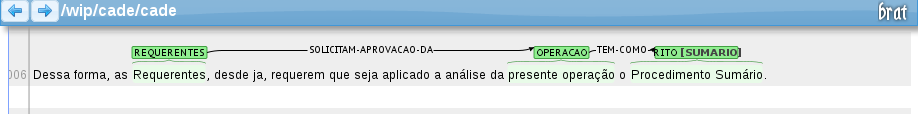
\includegraphics[scale=0.59]{brat}
\end{figure}

\begin{center}
  Figura 5.2: \textit{Screenshot} de anotações geradas manualmente no BRAT em um AC.
\end{center}

Na sequência, falaremos sobre Apache OpenNLP e como esta outra ferramenta foi utilizada no trabalho.

\section{Apache OpenNLP}

\indent\indent O Apache OpenNLP é um \textit{software} escrito e mantido pela \textit{Apache OpenNLP Development Community} distribuído sob a licença \textit{open source}
Apache 2.0 da Apache Software Foundation (ASF). Ele é uma biblioteca que contém uma série de ferramentas para processamento de linguagem natural baseadas em aprendizado
de máquina. As rotinas mais comuns de PLN, tais como tokenização, segmentação de sentenças, \textit{POS tagging}, reconhecimento de entidades mencionadas, \textit{chunking}
dentre outros. Sua meta é criar um arcabouço maduro para ferramentas de PLN mencionadas, além de distribuir modelos para serem usados com vários idiomas distintos bem como
a distribuição de texto anotados e modelos derivados destes.

Esta seção é reservada para falarmos das rotinas do OpenNLP que foram usados no desenvolvimento do trabalho
ao mesmo tempo que fornecemos exemplos de saídas geradas por ele com relação aos Atos de Concentração.


\subsection{Tokenizer}

\indent\indent Já tratamos sobre a questão do que é uma \textit{token} no Capítulo 3, e agora vamos explorar sobre a ferramenta de
tokenização fornecida pelo Apache OpenNLP. As implementações de tokenização oferecidas pelo Apache OpenNLP são as seguintes:

\begin{enumerate}[label=\textbf{{\Roman*.}}]
  \item Tokenizador de espaco em branco: identifica sequências de caracteres não brancos como \textit{tokens}.
  \item Tokenizador simples: identifica sequências de caracteres da mesma classe (como pontuações, digitos, alfabéticos etc) como \textit{tokens}.
  \item Tokenizador com aprendizado: usa modelos probabilísticos para identificar as fronteiras das \textit{tokens}. Tem base no método da máxima entropia.
\end{enumerate}

Finalmente, a tarefa de tokenização implementada no Apache OpenNLP é contituída de duas etapas distintas: identificação de fronteira de sentenças seguida da identificação das
tokens pertencentes à sentença encontrada, conforme já mencionado na nona nota de rodapé, na página 26.

Agora que já apresentamos as informações básicas do tokenizador, veremos alguns exemplos de saída. Considere o trecho abaixo, retirado do Ato de Concentração nº 08700.005269/2016-72:

\begin{quote}
  \textit{\quotes{19. Mas não é só isso. O prazo de exploração do bloco \hl{CAL-M-372} \hl{encontra-se} suspenso pela ANP desde \hl{16/05/2013} em razão de pendência no processo de obtenção de licença ambiental. Dessa forma, ainda não há previsão de quando essa pendência será solucionada ou de quando a exploração do bloco será retomada, o que corrobora a absoluta ausência de efeitos da operação sobre o mercado. Para fins de esclarecimento, nenhuma operação poderá ser realizada no Bloco enquanto não houver sido expedida a licença ambiental.}}
\end{quote}

Os exemplos 5.5 e 5.6 a seguir ilustram as saídas das implementações do tokenizador simples (\textbf{II}) e do tokenizador com aprendizado (\textbf{III}), respectivamente. Repare nas tokenizações que foram feitas com relação às \textit{tokens} grifadas em \hl{\textbf{amarelo}} no trecho destacado acima.

\begin{quote}
  \fbox{19} \fbox{.} \fbox{Mas} \fbox{não} \fbox{é} \fbox{só} \fbox{isso} \fbox{.} \fbox{O} \fbox{prazo} \fbox{de} \fbox{exploração} \fbox{do} \fbox{bloco} \fbox{CAL} \fbox{-}
\fbox{M} \fbox{-} \fbox{372} \fbox{encontra} \fbox{-} \fbox{se} \fbox{suspenso} \fbox{pela} \fbox{ANP} \fbox{desde} \fbox{16} \fbox{/} \fbox{05} \fbox{/} \fbox{2013} \fbox{em}
\fbox{razão} \fbox{de} \fbox{pendência} \fbox{no} \fbox{processo} \fbox{de} \fbox{obtenção} \fbox{de} \fbox{licença} \fbox{ambiental} \fbox{.} \fbox{Dessa} \fbox{forma} \fbox{,}
\fbox{ainda} \fbox{não} \fbox{há} \fbox{previsão} \fbox{de} \fbox{quando} \fbox{essa} \fbox{pendência} \fbox{será} \fbox{solucionada} \fbox{ou} \fbox{de} \fbox{quando} \fbox{a}
\fbox{exploração} \fbox{do} \fbox{bloco} \fbox{será} \fbox{retomada} \fbox{,} \fbox{o} \fbox{que} \fbox{corrobora} \fbox{a} \fbox{absoluta} \fbox{ausência} \fbox{de} \fbox{efeitos}
\fbox{da} \fbox{operação} \fbox{sobre} \fbox{o} \fbox{mercado} \fbox{.} \fbox{Para} \fbox{fins} \fbox{de} \fbox{esclarecimento} \fbox{,} \fbox{nenhuma} \fbox{operação} \fbox{poderá}
\fbox{ser} \fbox{realizada} \fbox{no} \fbox{Bloco} \fbox{enquanto} \fbox{não} \fbox{houver} \fbox{sido} \fbox{expedida} \fbox{a} \fbox{licença} \fbox{ambiental} \fbox{.}
\end{quote}
\begin{center}
  Exemplo 5.5: Saída do tokenizador do Apache OpenNLP usando a implementação do tokenizador simples.
\end{center}

\begin{quote}
  \fbox{19} \fbox{.} \fbox{Mas} \fbox{não} \fbox{é} \fbox{só} \fbox{isso} \fbox{.} \fbox{O} \fbox{prazo} \fbox{de} \fbox{exploração} \fbox{do} \fbox{bloco} \fbox{CAL-M-372} \fbox{encontra-se}
\fbox{suspenso} \fbox{pela} \fbox{ANP} \fbox{desde} \fbox{16/05/2013} \fbox{em} \fbox{razão} \fbox{de} \fbox{pendência} \fbox{no} \fbox{processo} \fbox{de} \fbox{obtenção} \fbox{de}
\fbox{licença} \fbox{ambiental} \fbox{.} \fbox{Dessa} \fbox{forma} \fbox{,} \fbox{ainda} \fbox{não} \fbox{há} \fbox{previsão} \fbox{de} \fbox{quando} \fbox{essa} \fbox{pendência} \fbox{será} \fbox{solucionada} \fbox{ou} \fbox{de} \fbox{quando} \fbox{a} \fbox{exploração} \fbox{do} \fbox{bloco} \fbox{será} \fbox{retomada} \fbox{,} \fbox{o} \fbox{que} \fbox{corrobora} \fbox{a} \fbox{absoluta} \fbox{ausência} \fbox{de} \fbox{efeitos} \fbox{da} \fbox{operação} \fbox{sobre} \fbox{o} \fbox{mercado} \fbox{.} \fbox{Para} \fbox{fins} \fbox{de} \fbox{esclarecimento} \fbox{,} \fbox{nenhuma} \fbox{operação} \fbox{poderá} \fbox{ser} \fbox{realizada} \fbox{no} \fbox{Bloco} \fbox{enquanto} \fbox{não} \fbox{houver} \fbox{sido} \fbox{expedida}
\fbox{a} \fbox{licença} \fbox{ambiental} \fbox{.}
\end{quote}
\begin{center}
  Exemplo 5.6: Saída do tokenizador do Apache OpenNLP usando a implementação do tokenizador com aprendizado.
\end{center}

Na seção a seguir veremos como o Apache OpenNLP trabalha com a tarefa de segmentação de sentenças.

\subsection{Sentence Detector}

\indent\indent Outra ferramenta que o Apache OpenNLP fornece, conforme já mencionado anteriormente, é um segmentador de sentenças capaz de detectar características textuais
tais como quando uma determinada pontuação marca o final de uma dada sentença ou não.

Para isso, conforme já discutido no Capítulo 3, existe uma
necessidade natural de definir o que é uma sentença. Para o segmentador de sentenças do Apache OpenNLP, uma sentença é definida como a maior sequência de caracteres entre duas
pontuações desconsiderando os caracteres de espaços em branco. As exceções à definição são a primeira e a última sentença, no qual no primeiro caso é assumido que o primeiro caractere que não
seja um espaço em branco marca o início da sentença, enquanto que no segundo caso o último caractere que não seja um espaço em branco é assumido como final da sentença.

A segmentação de
sentenças é o primeiro processo realizado pelo Apache OpenNLP, e é particularmente importante para o uso do \textit{software}, uma vez que a maior parte das ferramentas fornecidas esperam
entradas já quebradas em sentenças.

Consideremos mais uma vez o trecho extraído do Ato de Concentração nº 08700.005269/2016-72, que serviu de exemplo na seção anterior para ilustrar os exemplos 5.5 e 5.6:

\begin{quote}
  \textit{\quotes{19. Mas não é só isso. O prazo de exploração do bloco CAL-M-372 encontra-se suspenso pela ANP desde 16/05/2013 em razão de pendência no processo de obtenção de licença ambiental. Dessa forma, ainda não há previsão de quando essa pendência será solucionada ou de quando a exploração do bloco será retomada, o que corrobora a absoluta ausência de efeitos da operação sobre o mercado. Para fins de esclarecimento, nenhuma operação poderá ser realizada no Bloco enquanto não houver sido expedida a licença ambiental.}}
\end{quote}

Tal trecho, quando usado para alimentar a ferramenta de quebras de sentenças do Apache OpenNLP, gera a saída ilustrada no exemplo 5.7, exibido logo abaixo para o leitor:

\begin{quote}
  \fbox{
      \begin{varwidth}{0.86\textwidth}
      19.
      \end{varwidth}}
\end{quote}

\begin{quote}
  \fbox{
      \begin{varwidth}{0.86\textwidth}
      Mas não é só isso.
      \end{varwidth}}
\end{quote}

\begin{quote}
  \fbox{
      \begin{varwidth}{0.86\textwidth}
      O prazo de exploração do bloco CAL-M-372 encontra-se suspenso pela ANP desde 16/05/2013 em razão de pendência no processo de obtenção de licença ambiental.
      \end{varwidth}}
\end{quote}

\begin{quote}
  \fbox{
      \begin{varwidth}{0.86\textwidth}
      Dessa forma, ainda não há previsão de quando essa pendência será solucionada ou de quando a exploração do bloco será retomada, o que corrobora a absoluta ausência de efeitos da operação sobre o mercado.
      \end{varwidth}}
\end{quote}

\begin{quote}
  \fbox{
      \begin{varwidth}{0.86\textwidth}
      Para fins de esclarecimento, nenhuma operação poderá ser realizada no Bloco enquanto não houver sido expedida a licença ambiental.
      \end{varwidth}}
\end{quote}

\begin{center}
  Exemplo 5.7: Saída do segmentador de sentenças do Apache OpenNLP.
\end{center}

Finalmente, na próxima e última seção, falaremos sobre a ferramenta de REM fornecida pelo OpenNLP.

\pagebreak

\subsection{Name Finder}

\indent\indent A última ferramenta que foi usada para o desenvolvimento do trabalho disponibilizada pelo Apache OpenNLP é a \textit{Name Finder}, que faz o
reonhecimento de entidades mencionadas. Para usá-la, é necessário ter um modelo de REM criado no idioma correspondente. Nosso modelo, no caso, foi o córpus desenvolvido
a partir dos Atos de Concentração do CADE e manualmente anotados com uso do BRAT.

Para usar a ferramenta de REM, é necessário que se tenha modelos de detecção de sentença e tokenização criados previamente. Conforme já mencionado anteriormente nesta monografia,
idealmente deveríamos dispor de córpus de tokenização e detecção de sentenças criados em cima dos Atos de Concentração também, mas tal tarefa exigiria mais tempo que o
disponível, restando focarmos no desenvolvimento do córpus de REM (que é mais complexo) e aceitar os erros oriundos de modelos de baixa representatividade com relação
à tokenização e à detecção de sentenças, uma vez que estamos usando modelos treinados em cima de outras coleções de documentos e não dos nossos ACs selecionados.

Consideremos o trecho transcrito abaixo, retirado do Ato de Concentração nº , para avaliarmos a saída da ferramenta de REM do Apache OpenNLP. Ainda, considere
que a saída esperada tenha as seguintes anotações, representadas pelos \textit{frames} logo abaixo:

\begin{quote}
  \textit{``Pelo exposto, as \fbox{Requerentes}}$_{\text{Requerente}}$\textit{ submetem a \fbox{presente operação}}$_{\text{Operação}}$\textit{ para aprovação do \fbox{CADE}}$_{\text{Organização}}$\textit{, sem restrições,
  entendendo que a mesma nao resulta em
  concentração econômica, nao podendo, ainda que potencialmente, causar efeitos deletérios ao \fbox{mercado}}$_{\text{Mercado}}$\textit{ e ao bem—estar econômico da sociedade.
  Para tanto, requer-se que a \fbox{operação em tela}}$_{\text{Operation}}$\textit{ seja incondicionalmente aprovada, na forma da lei."}
\end{quote}

E abaixo, a resposta obtida, ilustrada no exemplo 5.8:

\begin{quote}
  \quotes{Pelo exposto, as \fbox{Requerentes}$_{\text{Requerente}}$ submetem a \fbox{presente operação}$_{\text{Operação}}$ para aprovação do \hl{\mbox{CADE}}, sem restrições,
  entendendo que a mesma nao resulta em concentração econômica, nao podendo, ainda que potencialmente, causar efeitos deletérios ao \fbox{mercado}$_{\text{Mercado}}$ e
  ao bem—estar econômico da sociedade. Para tanto, requer-se que a \hl{\mbox{operação em tela}} seja incondicionalmente aprovada, na forma da lei.}
\end{quote}
\begin{center}
  Exemplo 5.8: Saída do reconhecedor de EMs do Apache OpenNLP.
\end{center}

Notavelmente, temos 2 erros de saída com relação à fase de identificação, caracterizados pela perda das entidades. Acima, os termos \quotes{CADE} e \quotes{operação em tela}
grifados em \hl{\textbf{amarelo}} deveriam ter sido marcados com as etiquetas \quotes{Organização} e \quotes{Operação}, respectivamente.

No próximo capítulo serão apresentados os resultados obtidos do córpus desenvolvido, além de falarmos como os obtivemos.

\pagebreak
\chapter{Resultados}

\indent\indent Agora que os objetivos foram introduzidos, as teorias foram cobertas, o que foi desenvolvido foi abordado e as ferramentas que possibilitaram o desenvolvimento do trabalho
foram exploradas, podemos finalmente falar dos resultados obtidos com o córpus construído em cima dos Atos de Concentração Econômica do CADE. Neste capítulo, serão apresentados
valores de validação do córpus, a forma que obtivemos tais valores e comentários acerca dos valores.

\section{Validação Cruzada}

\indent\indent Para realizarmos os testes com o córpus foi usada a técnica de validação cruzada com o método \textit{holdout}. A idéia de usarmos a validação cruzada
é para testarmos a capacidade de generalização do nosso modelo a partir dos dados do nosso córpus anotado e assim ganharmos também mais garantia acerca da sua robustez.

O incentivo para que o método de \textit{holdout} tenha sido usado
é que como não dispunhamos de muitos dados (no sentido de que o córpus possui apenas pouco mais de 50000 palavras quando idealmente havia uma meta de 300000 palavras), dividirmos o córpus composto de 50 ACs
em um grupo de treinamento composto de 45 processos e um segundo grupo composto dos 5 restantes para o grupo de teste pareceu uma aproximação mais razoável, uma vez que a quantidade de palavras
continuaria sendo suficientemente grande no grupo de treinamento (cerca de 45000) e ainda restaria 10\% do total que poderia ser usado para fazermos a validação. Como, porém, este é um
método que pode ter alta variância, foram feito 10 casos distintos, onde os grupos de treinamento e de teste são compostos por ACs diferentes.

Na tabela 6.3 a seguir, são apresentadas as $C_i, 1 \leq i \leq 10$ combinações dos $A_j, 1 \leq j \leq 50$ que foram selecionadas pseudo-aleatoriamente a partir de \textit{script} para compôr os grupos de treinamento e de teste. As tabelas 6.1 e 6.2 abaixo mostram a atribuição de um valor \textit{j} para um AC.


\begin{table}[h!]
  \centering
  \hspace*{-2.15cm}
  \def\arraystretch{1.1}
  \begin{tabular}{| c | c || c | c || c | c || c | c |}
    \hline
    \multicolumn{8}{| c |}{Ordinários} \\
    \hline
    \textit{j} & Nº Processo & \textit{j} & Nº Processo & \textit{j} & Nº Processo & \textit{j} & Nº Processo \\
    \hline\hline
    1 & 08700.000722/2016-54 & 8  & 08700.003045/2016-26 & 15 & 08700.004211/2016-10 & 22 & 08700.005683/2016-81 \\
    2 & 08700.000723/2016-07 & 9  & 08700.003252/2016-81 & 16 & 08700.004360/2016-71 & 23 & 08700.005702/2016-70 \\
    3 & 08700.001221/2016-95 & 10 & 08700.003421/2016-82 & 17 & 08700.004557/2016-18 & 24 & 08700.005733/2016-21 \\
    4 & 08700.001872/2016-85 & 11 & 08700.003462/2016-79 & 18 & 08700.004860/2016-11 & 25 & 08700.010790/2015-41 \\
    5 & 08700.002432/2016-45 & 12 & 08700.003636/2016-01 & 19 & 08700.005093/2016-59 & &  \\
    6 & 08700.002792/2016-47 & 13 & 08700.003952/2016-75 & 20 & 08700.005398/2016-61 & &  \\
    7 & 08700.003024/2016-19 & 14 & 08700.004168/2016-84 & 21 & 08700.005524/2016-87 & &  \\
    \hline
    \end{tabular}
  \caption{ACs Ordinários que compõem o córpus e seus respectivos número \textit{j}.}
\end{table}

\begin{table}[h!]
  \centering
  \hspace*{-2.25cm}
  \def\arraystretch{1.1}
  \begin{tabular}{| c | c || c | c || c | c || c | c |}
    \hline
    \multicolumn{8}{| c |}{Sumários} \\
    \hline
    \textit{j} & Nº Processo & \textit{j} & Nº Processo & \textit{j} & Nº Processo & \textit{j} & Nº Processo \\
    \hline\hline
    26 & 08700.000625/2016-61 & 33 & 08700.005002/2016-85 & 40 & 08700.005334/2016-60 & 47 & 08700.005603/2016-98 \\
    27 & 08700.001192/2016-61 & 34 & 08700.005138/2016-95 & 41 & 08700.005387/2016-81 & 48 & 08700.005619/2016-09 \\
    28 & 08700.003684/2016-91 & 35 & 08700.005139/2016-30 & 42 & 08700.005456/2016-56 & 49 & 08700.005620/2016-25 \\
    29 & 08700.003951/2016-21 & 36 & 08700.005204/2016-27 & 43 & 08700.005457/2016-09 & 50 & 08700.005667/2016-99 \\
    30 & 08700.004768/2016-42 & 37 & 08700.005208/2016-13 & 44 & 08700.005559/2016-16 &    & \\
    31 & 08700.004963/2016-72 & 38 & 08700.005259/2016-37 & 45 & 08700.005580/2016-11 &    & \\
    32 & 08700.005000/2016-96 & 39 & 08700.005269/2016-72 & 46 & 08700.005587/2016-33 &    & \\
   \hline
  \end{tabular}
  \caption{ACs Sumários que compõem o córpus e seus respectivos número \textit{j}.}
\end{table}

\begin{table}[h!]
  \centering
  \def\arraystretch{0.475}
  \begin{tabular}{| c | c | c | c | c | c | c | c | c | c | c |}
    \hline
    \backslashbox{\small{$A_j$}}{\small{$C_i$}} & \small{$C_1$} & \small{$C_2$} & \small{$C_3$} & \small{$C_4$} & \small{$C_5$} & \small{$C_6$} & \small{$C_7$} & \small{$C_8$} & \small{$C_9$} & \small{$C_{10}$} \\
    \hline
    \small{$A_1$}  & \cellcolor{train} & \cellcolor{train} & \cellcolor{train} & \cellcolor{train} & \cellcolor{train} & \cellcolor{train} & \cellcolor{test}  & \cellcolor{train} & \cellcolor{train} &  \cellcolor{train} \\ \hline
    \small{$A_2$}  & \cellcolor{train} & \cellcolor{train} & \cellcolor{test}  & \cellcolor{train} & \cellcolor{train} & \cellcolor{test}  & \cellcolor{train} & \cellcolor{test}  & \cellcolor{train} &  \cellcolor{train} \\ \hline
    \small{$A_3$}  & \cellcolor{train} & \cellcolor{train} & \cellcolor{train} & \cellcolor{train} & \cellcolor{train} & \cellcolor{train} & \cellcolor{train} & \cellcolor{train} & \cellcolor{train} &  \cellcolor{train} \\ \hline
    \small{$A_4$}  & \cellcolor{train} & \cellcolor{train} & \cellcolor{train} & \cellcolor{test}  & \cellcolor{train} & \cellcolor{train} & \cellcolor{train} & \cellcolor{train} & \cellcolor{train} &  \cellcolor{train} \\ \hline
    \small{$A_5$}  & \cellcolor{train} & \cellcolor{train} & \cellcolor{train} & \cellcolor{train} & \cellcolor{train} & \cellcolor{train} & \cellcolor{train} & \cellcolor{train} & \cellcolor{test}  &  \cellcolor{train} \\ \hline
    \small{$A_6$}  & \cellcolor{test}  & \cellcolor{test}  & \cellcolor{train} & \cellcolor{train} & \cellcolor{train} & \cellcolor{train} & \cellcolor{train} & \cellcolor{train} & \cellcolor{train} &  \cellcolor{train} \\ \hline
    \small{$A_7$}  & \cellcolor{train} & \cellcolor{train} & \cellcolor{train} & \cellcolor{test}  & \cellcolor{train} & \cellcolor{train} & \cellcolor{train} & \cellcolor{train} & \cellcolor{train} &  \cellcolor{train} \\ \hline
    \small{$A_8$}  & \cellcolor{train} & \cellcolor{train} & \cellcolor{train} & \cellcolor{train} & \cellcolor{train} & \cellcolor{train} & \cellcolor{train} & \cellcolor{train} & \cellcolor{train} &  \cellcolor{train} \\ \hline
    \small{$A_9$}  & \cellcolor{train} & \cellcolor{train} & \cellcolor{train} & \cellcolor{train} & \cellcolor{train} & \cellcolor{train} & \cellcolor{test}  & \cellcolor{train} & \cellcolor{train} &  \cellcolor{train} \\ \hline
    \small{$A_{10}$} & \cellcolor{train} & \cellcolor{test}  & \cellcolor{train} & \cellcolor{train} & \cellcolor{train} & \cellcolor{train} & \cellcolor{train} & \cellcolor{train} & \cellcolor{train} &  \cellcolor{train} \\ \hline
    \small{$A_{11}$} & \cellcolor{train} & \cellcolor{train} & \cellcolor{train} & \cellcolor{train} & \cellcolor{train} & \cellcolor{train} & \cellcolor{train} & \cellcolor{train} & \cellcolor{train} & \cellcolor{test}  \\ \hline
    \small{$A_{12}$} & \cellcolor{train} & \cellcolor{train} & \cellcolor{train} & \cellcolor{train} & \cellcolor{train} & \cellcolor{train} & \cellcolor{train} & \cellcolor{train} & \cellcolor{train} &  \cellcolor{train} \\ \hline
    \small{$A_{13}$} & \cellcolor{train} & \cellcolor{train} & \cellcolor{train} & \cellcolor{train} & \cellcolor{train} & \cellcolor{train} & \cellcolor{train} & \cellcolor{train} & \cellcolor{train} &  \cellcolor{train} \\ \hline
    \small{$A_{14}$} & \cellcolor{train} & \cellcolor{train} & \cellcolor{train} & \cellcolor{train} & \cellcolor{test}  & \cellcolor{train} & \cellcolor{train} & \cellcolor{train} & \cellcolor{train} &  \cellcolor{train} \\ \hline
    \small{$A_{15}$} & \cellcolor{train} & \cellcolor{train} & \cellcolor{test}  & \cellcolor{train} & \cellcolor{train} & \cellcolor{train} & \cellcolor{train} & \cellcolor{train} & \cellcolor{train} & \cellcolor{test}  \\ \hline
    \small{$A_{16}$} & \cellcolor{train} & \cellcolor{train} & \cellcolor{train} & \cellcolor{train} & \cellcolor{train} & \cellcolor{train} & \cellcolor{train} & \cellcolor{train} & \cellcolor{train} &  \cellcolor{train} \\ \hline
    \small{$A_{17}$} & \cellcolor{train} & \cellcolor{train} & \cellcolor{train} & \cellcolor{train} & \cellcolor{train} & \cellcolor{train} & \cellcolor{train} & \cellcolor{train} & \cellcolor{train} &  \cellcolor{train} \\ \hline
    \small{$A_{18}$} & \cellcolor{train} & \cellcolor{train} & \cellcolor{train} & \cellcolor{train} & \cellcolor{train} & \cellcolor{train} & \cellcolor{train} & \cellcolor{train} & \cellcolor{train} &  \cellcolor{train} \\ \hline
    \small{$A_{19}$} & \cellcolor{train} & \cellcolor{train} & \cellcolor{train} & \cellcolor{train} & \cellcolor{train} & \cellcolor{train} & \cellcolor{train} & \cellcolor{train} & \cellcolor{train} &  \cellcolor{train} \\ \hline
    \small{$A_{20}$} & \cellcolor{train} & \cellcolor{train} & \cellcolor{train} & \cellcolor{train} & \cellcolor{train} & \cellcolor{train} & \cellcolor{train} & \cellcolor{train} & \cellcolor{train} &  \cellcolor{train} \\ \hline
    \small{$A_{21}$} & \cellcolor{train} & \cellcolor{train} & \cellcolor{train} & \cellcolor{test}  & \cellcolor{train} & \cellcolor{train} & \cellcolor{train} & \cellcolor{train} & \cellcolor{train} &  \cellcolor{train} \\ \hline
    \small{$A_{22}$} & \cellcolor{train} & \cellcolor{train} & \cellcolor{train} & \cellcolor{train} & \cellcolor{train} & \cellcolor{train} & \cellcolor{test}  & \cellcolor{train} & \cellcolor{train} &  \cellcolor{train} \\ \hline
    \small{$A_{23}$} & \cellcolor{train} & \cellcolor{train} & \cellcolor{train} & \cellcolor{train} & \cellcolor{train} & \cellcolor{test}  & \cellcolor{train} & \cellcolor{train} & \cellcolor{train} &  \cellcolor{train} \\ \hline
    \small{$A_{24}$} & \cellcolor{train} & \cellcolor{train} & \cellcolor{train} & \cellcolor{train} & \cellcolor{train} & \cellcolor{train} & \cellcolor{train} & \cellcolor{train} & \cellcolor{train} &  \cellcolor{train} \\ \hline
    \small{$A_{25}$} & \cellcolor{test}  & \cellcolor{train} & \cellcolor{train} & \cellcolor{train} & \cellcolor{train} & \cellcolor{train} & \cellcolor{train} & \cellcolor{train} & \cellcolor{train} &  \cellcolor{train} \\ \hline
    \small{$A_{26}$} & \cellcolor{train} & \cellcolor{train} & \cellcolor{train} & \cellcolor{train} & \cellcolor{train} & \cellcolor{train} & \cellcolor{train} & \cellcolor{train} & \cellcolor{train} &  \cellcolor{train} \\ \hline
    \small{$A_{27}$} & \cellcolor{train} & \cellcolor{train} & \cellcolor{train} & \cellcolor{test}  & \cellcolor{train} & \cellcolor{train} & \cellcolor{train} & \cellcolor{train} & \cellcolor{train} &  \cellcolor{train} \\ \hline
    \small{$A_{28}$} & \cellcolor{train} & \cellcolor{test}  & \cellcolor{train} & \cellcolor{train} & \cellcolor{train} & \cellcolor{train} & \cellcolor{train} & \cellcolor{train} & \cellcolor{test}  &  \cellcolor{train} \\ \hline
    \small{$A_{29}$} & \cellcolor{train} & \cellcolor{test}  & \cellcolor{train} & \cellcolor{train} & \cellcolor{train} & \cellcolor{train} & \cellcolor{train} & \cellcolor{train} & \cellcolor{train} &  \cellcolor{train} \\ \hline
    \small{$A_{30}$} & \cellcolor{train} & \cellcolor{train} & \cellcolor{train} & \cellcolor{train} & \cellcolor{test}  & \cellcolor{train} & \cellcolor{train} & \cellcolor{train} & \cellcolor{train} & \cellcolor{test}  \\ \hline
    \small{$A_{31}$} & \cellcolor{train} & \cellcolor{train} & \cellcolor{train} & \cellcolor{train} & \cellcolor{train} & \cellcolor{train} & \cellcolor{test}  & \cellcolor{train} & \cellcolor{test}  &  \cellcolor{train} \\ \hline
    \small{$A_{32}$} & \cellcolor{test}  & \cellcolor{train} & \cellcolor{test}  & \cellcolor{train} & \cellcolor{train} & \cellcolor{train} & \cellcolor{train} & \cellcolor{train} & \cellcolor{train} &  \cellcolor{train} \\ \hline
    \small{$A_{33}$} & \cellcolor{train} & \cellcolor{train} & \cellcolor{train} & \cellcolor{train} & \cellcolor{test}  & \cellcolor{train} & \cellcolor{train} & \cellcolor{train} & \cellcolor{train} &  \cellcolor{train} \\ \hline
    \small{$A_{34}$} & \cellcolor{train} & \cellcolor{train} & \cellcolor{train} & \cellcolor{train} & \cellcolor{test}  & \cellcolor{train} & \cellcolor{train} & \cellcolor{train} & \cellcolor{test}  &  \cellcolor{train} \\ \hline
    \small{$A_{35}$} & \cellcolor{train} & \cellcolor{test}  & \cellcolor{train} & \cellcolor{train} & \cellcolor{train} & \cellcolor{train} & \cellcolor{train} & \cellcolor{train} & \cellcolor{train} &  \cellcolor{train} \\ \hline
    \small{$A_{36}$} & \cellcolor{train} & \cellcolor{train} & \cellcolor{train} & \cellcolor{train} & \cellcolor{train} & \cellcolor{train} & \cellcolor{train} & \cellcolor{train} & \cellcolor{train} &  \cellcolor{train} \\ \hline
    \small{$A_{37}$} & \cellcolor{train} & \cellcolor{train} & \cellcolor{test}  & \cellcolor{train} & \cellcolor{train} & \cellcolor{train} & \cellcolor{train} & \cellcolor{train} & \cellcolor{train} & \cellcolor{test}  \\ \hline
    \small{$A_{38}$} & \cellcolor{train} & \cellcolor{train} & \cellcolor{train} & \cellcolor{train} & \cellcolor{test}  & \cellcolor{train} & \cellcolor{train} & \cellcolor{train} & \cellcolor{train} &  \cellcolor{train} \\ \hline
    \small{$A_{39}$} & \cellcolor{train} & \cellcolor{train} & \cellcolor{train} & \cellcolor{train} & \cellcolor{train} & \cellcolor{train} & \cellcolor{train} & \cellcolor{test}  & \cellcolor{train} &  \cellcolor{train} \\ \hline
    \small{$A_{40}$} & \cellcolor{test}  & \cellcolor{train} & \cellcolor{train} & \cellcolor{train} & \cellcolor{train} & \cellcolor{train} & \cellcolor{train} & \cellcolor{train} & \cellcolor{train} &  \cellcolor{train} \\ \hline
    \small{$A_{41}$} & \cellcolor{train} & \cellcolor{train} & \cellcolor{test}  & \cellcolor{test}  & \cellcolor{train} & \cellcolor{train} & \cellcolor{train} & \cellcolor{train} & \cellcolor{train} &  \cellcolor{train} \\ \hline
    \small{$A_{42}$} & \cellcolor{train} & \cellcolor{train} & \cellcolor{train} & \cellcolor{train} & \cellcolor{train} & \cellcolor{test}  & \cellcolor{train} & \cellcolor{train} & \cellcolor{test}  &  \cellcolor{train} \\ \hline
    \small{$A_{43}$} & \cellcolor{train} & \cellcolor{train} & \cellcolor{train} & \cellcolor{train} & \cellcolor{train} & \cellcolor{train} & \cellcolor{train} & \cellcolor{test}  & \cellcolor{train} & \cellcolor{test}  \\ \hline
    \small{$A_{44}$} & \cellcolor{test}  & \cellcolor{train} & \cellcolor{train} & \cellcolor{train} & \cellcolor{train} & \cellcolor{test}  & \cellcolor{train} & \cellcolor{test}  & \cellcolor{train} &  \cellcolor{train} \\ \hline
    \small{$A_{45}$} & \cellcolor{train} & \cellcolor{train} & \cellcolor{train} & \cellcolor{train} & \cellcolor{train} & \cellcolor{test}  & \cellcolor{train} & \cellcolor{train} & \cellcolor{train} &  \cellcolor{train} \\ \hline
    \small{$A_{46}$} & \cellcolor{train} & \cellcolor{train} & \cellcolor{train} & \cellcolor{train} & \cellcolor{train} & \cellcolor{train} & \cellcolor{train} & \cellcolor{train} & \cellcolor{train} &  \cellcolor{train} \\ \hline
    \small{$A_{47}$} & \cellcolor{train} & \cellcolor{train} & \cellcolor{train} & \cellcolor{train} & \cellcolor{train} & \cellcolor{train} & \cellcolor{train} & \cellcolor{test}  & \cellcolor{train} &  \cellcolor{train} \\ \hline
    \small{$A_{48}$} & \cellcolor{train} & \cellcolor{train} & \cellcolor{train} & \cellcolor{train} & \cellcolor{train} & \cellcolor{train} & \cellcolor{train} & \cellcolor{train} & \cellcolor{train} &  \cellcolor{train} \\ \hline
    \small{$A_{49}$} & \cellcolor{train} & \cellcolor{train} & \cellcolor{train} & \cellcolor{train} & \cellcolor{train} & \cellcolor{train} & \cellcolor{test}  & \cellcolor{train} & \cellcolor{train} &  \cellcolor{train} \\ \hline
    \small{$A_{50}$} & \cellcolor{train} & \cellcolor{train} & \cellcolor{train} & \cellcolor{train} & \cellcolor{train} & \cellcolor{train} & \cellcolor{train} & \cellcolor{train} & \cellcolor{train} &  \cellcolor{train} \\ \hline
  \end{tabular}
  \begin{tabular}{| c | c |}
    \hline
    \cellcolor{train} & Treinamento \\ \hline
    \cellcolor{test} & Teste \\ \hline
  \end{tabular}
  \caption{Composição dos grupos de treinamento e teste de cada combinação $C_i$}
\end{table}

\subsection{Obtendo Valores}

\indent\indent Uma vez com os grupos de treinamento e de teste determinados, podemos fazer estimativas com o córpus usando as métricas. Para isso, precisamos
apenas obter as quantidades de acertos e erros em relação à resposta esperada. Fazemos isso da seguinte forma:


\begin{itemize}
  \item Para cada $C_i, 1 \leq i \leq 10$, treinamos um modelo de REM no Apache OpenNLP usando as anotações BRAT dos 45 ACs do grupo de treinamento e depois, usando modelo, marcamos
o grupo de teste de forma automatizada e comparamos as anotações geradas com as anotações originais do grupo de teste.
  \item Efetuadas as computações de treinamento e geração de anotações, contabilizamos as quantidades de acertos e de erros de cada uma das 10 combinações $C_i$.
  \item Foram consideradas 3 categorias de erro:
  \begin{enumerate}[label={\textbf{E\arabic*.}}]
    \item Entidades mencionadas perdidas (não identificadas).
    \item Entidades mencionadas com etiquetas erradas.
    \item Entidades mencionadas com erros posicionais (isto é, incluiu ou deixou de incluir palavras que deveriam ser consideradas em uma dada marcação).
  \end{enumerate}
  \item São verdadeiros positivos (\textbf{VP}) os acertos \textbf{A}.
  \item São falsos negativos (\textbf{FN}) os erros \textbf{E1} e \textbf{E3}, ou seja, \textbf{FN} = \textbf{E1} + \textbf{E3}.
  \item São falsos positivos (\textbf{FP}) os erros \textbf{E2} e \textbf{E3}, ou seja, \textbf{FP} = \textbf{E2} + \textbf{E3}.
  \item São verdadeiros negativos (\textbf{VN}) todas as \textit{tokens} que não eram EMs e, de fato, não foram recuperadas. Não há necessidade de contabilizar essa categoria.
  \item Chamamos de \textbf{R} (= \textbf{A} + \textbf{E2} + \textbf{E3}) o número de EMs que foram recuperadas naquela dada combinação e de \textbf{T} (= \textbf{A} + \textbf{E1} + \textbf{E3}) o número total de EMs que deveriam ser marcadas e recuperadas.
  \item Aplicamos o cálculo das métricas de Precisão (\textbf{P}), Cobertura (\textbf{C}) e Medida-F balanceada (\textbf{F$_1$}) usando os valores obtidos acima de \textbf{VP}, \textbf{FN}, \textbf{FP}, \textbf{VN}, \textbf{R} e \textbf{T} para cada uma das $C_i$ combinações.
\end{itemize}

Os valores obtidos para cada uma das combinações $C_i$ estão descritos na tabela a seguir para cada uma das categorias \textit{L}:

\begin{table}[h!]
  \centering
  \hspace*{-2.1cm}
  \def\arraystretch{1.1}
  \begin{tabular}{| P{1.45cm} | P{1.36cm} | P{1.36cm} | P{1.36cm} | P{1.36cm} | P{1.36cm} | P{1.36cm} | P{1.36cm} | P{1.36cm} | P{1.36cm} | P{1.36cm} |}
    \hline
    \backslashbox[19.1mm]{\textit{L}}{$C_i$} & $C_1$ & $C_2$ & $C_3$ & $C_4$ & $C_5$ & $C_6$ & $C_7$ & $C_8$ & $C_9$ & $C_{10}$ \\
    \hline
    \small{\textbf{R}}                 & \small{327} & \small{263} & \small{218} & \small{324} & \small{293} & \small{210} & \small{270} & \small{263} & \small{220} & \small{243} \\ \hline
    \small{\textbf{T}}                 & \small{774} & \small{527} & \small{491} & \small{741} & \small{653} & \small{520} & \small{702} & \small{623} & \small{587} & \small{605} \\ \hline
    \small{\textbf{A}}   & \small{258} & \small{208} & \small{168} & \small{248} & \small{231} & \small{162} & \small{208} & \small{210} & \small{179} & \small{184} \\ \hline
    \small{\textbf{E1} + \textbf{E3}} & \small{461 + 55} & \small{272 + 47} & \small{286 + 37} & \small{431 + 62} & \small{379 + 43} & \small{323 + 35} & \small{443 + 51} & \small{371 + 42} & \small{375 + 33} & \small{375 + 46} \\ \hline
    \small{\textbf{E2} + \textbf{E3}} & \small{14 + 55} & \small{8 + 47} & \small{13 + 37} & \small{14 + 62} & \small{19 + 43} & \small{13 + 35} & \small{11 + 51} & \small{11 + 42} & \small{8 + 33} & \small{13 + 46} \\ \hline\hline
    \small{\textbf{P}} & \small{0.789} & \small{0.790} & \small{0.770} & \small{0.765} & \small{0.788} & \small{0.771} & \small{0.770} & \small{0.798} & \small{0.813} & \small{0.757} \\ \hline
    \small{\textbf{C}} & \small{0.333} & \small{0.394} & \small{0.342} & \small{0.334} & \small{0.353} & \small{0.311} & \small{0.296} & \small{0.337} & \small{0.305} & \small{0.304} \\ \hline
\small{\textbf{F$_1$}} & \small{0.468} & \small{0.525} & \small{0.473} & \small{0.465} & \small{0.487} & \small{0.443} & \small{0.427} & \small{0.473} & \small{0.443} & \small{0.433} \\ \hline
    \end{tabular}
  \caption{Valores obtidos para cada $C_i$ em cada uma das categorias.}
\end{table}

Note que \textbf{E3} faz tanto parte de \textbf{FN} quanto de \textbf{FP}. A razão dele fazer parte de \textbf{FN} é porque parte da marcação é relevante, mas como está com limites imprecisos, devemos considerar como não recuperada. Já com relação a \textbf{FP}, como ele foi recuperado com erro de fronteira de marcação, devemos considerar que não é relevante.

\subsection{Interpretação}

\indent\indent Os resultados obtidos, expostos na tabela 6.4, nos revelam taxas que podem ser melhoradas. Em particular, é importante ressaltar 2 pontos:

\begin{enumerate}[label={\textbf{\arabic*.}}]
\item Os resultados obtidos foram feitos a partir de um córpus relativamente pequeno, o que justifica os valores baixo das taxas de cobertura de todas as combinações $C_i$.
\item Considerando a figura 5.1, é importante perceber que apenas 1 ciclo foi concluído. O \textit{loop} em busca do refinamento dos resultados deveria ser reiniciado considerando os
valores obtidos. Isso melhoraria as taxas de precisão de cobertura e consequentemente da Medida-F.
\end{enumerate}

É muito claro que o fato do córpus ser pequeno favoreceu um desbalanceamento entre as taxas de precisão e de cobertura, de tal modo que se ele fosse maior, mais entidades mencionadas
seriam identificadas, reduzindo o valor de \textbf{E1}, enquanto em contrapartida, ao identificar mais \textit{tokens} candidatas a anotações, poderíamos aumentar o valor de \textbf{E2}, afetando um pouco a precisão. Note, porém, que supondo que o processo fosse bem feito, a introdução de possíveis erros do tipo \textbf{E2} não seria um problema comparado à redução dos
erros do tipo \textbf{E1}.

Ainda, é importante considerar os erros humanos envolvidos no processo de anotação de entidades mencionadas no córpus, que pode gerar imprecisão. Idealmente, convém que mais
pessoas trabalhem no processo de anotação, revisando o conteúdo produzido pelo(s) anotador(es). Além disso, não podemos ignorar os eventuais erros de OCR que não foram corrigidos
e acabam impactando diretamente nos processos de tokenização e detecção de sentenças introduzindo possíveis erros que consequentemente afetam consideravelmente o processo de REM.

Os valores da Medida-F da tabela 6.4 nos mostram que a estimativa de erro, considerando nossas amostras diferentes, é em média de $\mu_{E} = 1 - \mu_{F_1} = 0.5363$. Em outras palavras,
considerando tanto os valores de precisão quanto os valores de cobertura, nosso córpus quase tem um desempenho mediano (50\%) no sentido de cobrir a coleção de Atos de Concentração Econômica precisamente.

\pagebreak
\chapter{Conclusão}

\indent\indent Tratar volumes muito grandes de dados é uma tarefa bastante trabalhosa e longe de ser trivial. É necessário, primeiramente, saber de todo o contexto
em que estes dados são gerados para, então, arriscar-se a entendê-los e partir para a identificação de quais possíveis informações sejam relevantes à tarefa que se deseja realizar. Nesse sentido, apesar de o objetivo inicial de classificação dos ritos não ter sido cumprido, um grande
aprendizado ficou com relação à tarefa de extrair informações de um grande volume de dados, além de um córpus que pode servir de base ou exemplo para aplicações futuras.

Em particular, com relação aos resultados, considerando a até então inexperiência do autor no que diz respeito a mexer com todas essas ferramentas e teorias abordadas nessa monografia,
é mais que satisfatório ter obtido valores de taxa de precisão cujo a média é superior a 75\% e quase atingir uma média de 50\% para a Medida-F. Entretanto, apesar de o trabalho desenvolvido aqui ter sido um grande passo numa possível direção correta para solucionar o problema proposto, ainda há muito a ser realizado no sentido de melhorar a qualidade do córpus construído, buscando refinar os resultados obtidos.

Finalmente, é importante considerar também a questão da interdisciplinaridade: o autor jamais teve qualquer contato com a área do direito econômico e houve a necessidade de dedicar horas
de estudo a este diferente universo para poder compreender o contexto em que os dados estão inseridos e então buscar extrair as melhores informações possíveis.

\section{Dificuldades encontradas}

\indent\indent São listadas a seguir algumas das dificuldades encontradas:

\begin{enumerate}[label={\textbf{\arabic*.}}]
  \item Identificar os dados potencialmente relevantes em meio a um grande volume de dados.
  \item Identificar nos dados uma estratégia que (talvez) solucione o desafio proposto.
  \item Idioma: a maior parte das ferramentas, modelos e textos providenciados são para o inglês.
  \item O próprio ato de anotar quando não se tem qualquer experiência, gerando sempre resquícios de dúvidas do quão correto a tarefa está sendo realizada. Como é necessário
um volume suficientemente grande de anotações, demorou uns meses para ter a primeira resposta.
  \item A falta de um especialista do direito econômico para trabalhar em conjunto no processo de anotações ou mesmo a falta de um texto gerado por um especialista que pudesse ser
o real documento padrão-ouro.
  \item Acostumar-se com as ferramentas.
  \item A falta de modelos de alta representatividade para os processos de tokenização e detecção de sentenças e a falta de tempo para desenvolvê-los também.
  \item O tratamento da \quotes{sujeira} gerado pelo OCR na hora de montar o córpus, uma vez que 100\% dos documentos de leitura estão em formato pdf.
\end{enumerate}

\section{Próximo Passo}

\indent\indent O próximo passo a ser seguido seria, antes de tudo, engordar o córpus com cerca de mais 250 Atos de Concentração para atingir cerca de 300 mil palavras e anotá-lo
na sequência. Em seguida, refinar os resultados seguindo o procedimento descrito na figura 5.1. Depois, achar um método de alimentar uma Rede Neural (ou algum outro método como Máquina de
Vetores de Suporte) com as entidades mencionadas encontradas sem que haja perda de informações (precisaríamos considerar o contexto em que as informações foram retiradas e seus relacionamentos) para, então, atribuirmos um ou outro tipo de rito. Este último passo é particularmente difícil de resolver, uma vez que o vetor de entrada da rede neural deveria ser
muito bem pensado de forma a não desperdiçar o valor das EMs.

\pagebreak
\chapter*{Referências}
\markboth{UNNUMBERED CHAPTER}{}

\begin{enumerate}[label={[\arabic*]}]
\item Acesso à Informação: Conheça o CADE. Disponível em: $\langle$ http://www.cade.gov.br/acesso-a-informacao/institucional $\rangle$. Acesso em: 13 de outubro de 2016.
\item Assessoria de Comunicação Social. Acesso à Informação: Histórico do CADE. Disponível em: $\langle$ http://www.cade.gov.br/acesso-a-informacao/institucional/historico-do-cade $\rangle$. Acesso em: 13 de outubro de 2016.
\item Assessoria de Comunicação Social. FAQ sobre Atos de Concentração Econômica. Disponível em: $\langle$ http://www.cade.gov.br/servicos/perguntas-frequentes/perguntas-sobre-atos-de-concentracao-economica $\rangle$. Acesso em: 14 de outubro de 2016.
\item Base de Dados pública do CADE: Pesquisa Processual. Disponível em: \newline$\langle$ http://www.cade.gov.br/assuntos/processos-1 $\rangle$. Acesso em: 14 de outubro de 2016.
\item Documentação Apache OpenNLP: REM. Disponível em: \newline$\langle$ https://opennlp.apache.org/documentation/1.6.0/manual/opennlp.html $\rangle$. \newline Acesso em: 14 de outubro de 2016.
\item CADE. Resolução nº 2, de 29 de maio de 2012. Disponível em: \newline$\langle$ http://www.cade.gov.br/assuntos/normas-e-legislacao/resolucao/resolucao-2\_2012-analise-atos-concentracao.pdf $\rangle$. Acesso em: 14 de outubro de 2016.
\item WIKIPEDIA. Natural Language Processing. Disponível em: \newline$\langle$ https://en.wikipedia.org/wiki/Natural\_language\_processing $\rangle$. Acesso em: 15 de outubro de 2016.
\item WIKIPEDIA. Brown Corpus. Disponível em: $\langle$ https://en.wikipedia.org/wiki/Brown\_Corpus $\rangle$. Acesso em: 15 de outubro de 2016.
\item SAMPSON, Geoffrey. The Susanne Corpus. Disponível em: \newline$\langle$ http://www.essex.ac.uk/linguistics/external/clmt/w3c/corpus\_ling/content/\newline corpora/list/public/susanne.html $\rangle$. Acesso em: 15 de outubro de 2016.
\item MANNING, Christopher D., SCHUETZE, Hinrich. Foundations of Statistical Natural Language Processing, MIT Press. Cambridge, MA: May 1999.
\item LINGUATECA. Corpus Amazônia. Disponível em $\langle$ http://www.linguateca.pt/floresta/\newline corpus.html\#amazonia $\rangle$. Acesso em: 15 de outrobro de 2016.
\item WIKIPEDIA. Sentence Boundary Disambiguation. Disponível em \newline$\langle$ https://en.wikipedia.org/wiki/Sentence\_boundary\_disambiguation $\rangle$. Acesso em: 19 de outubro de 2016.
\item INDURKHYA, Nitin., DAMERAU, Fred J., Handbook of Natural Language Processing, Chapman \& Hall/CRC, 2010.
\item CARVALHO, Wesley Seidel. Reconhecimento de entidades mencionadas em português utilizando aprendizado de máquina, São Paulo, 2012
\item WIKIPEDIA. Named Entity. Disponível em: $\langle$ https://en.wikipedia.org/wiki/Named\_entity $\rangle$. Acesso em: 22 de outubro de 2016.
\item WIKIPEDIA. Named Entity Recognition. Disponível em: \newline$\langle$ https://en.wikipedia.org/wiki/Named-entity\_recognition $\rangle$. Acesso em: 22 de outubro de 2016.
\item WIKIPEDIA. Gold-standard. Disponível em: \newline$\langle$ https://en.wikipedia.org/wiki/Gold\_standard\_\%28test\%29 $\rangle$. Acesso em: 23 de outubro de 2016.
\item MANNING, Christopher D., RAGHAVAN, Prabhakar., SCHUETZE, Hinrich. An Introduction to Information Retrieval. Online Edition. Cambridge University Press. 2008.
\item Pontus Stenetorp, Sampo Pyysalo, Goran Topić, Tomoko Ohta, Sophia Ananiadou and Jun'ichi Tsujii (2012). brat: a Web-based Tool for NLP-Assisted Text Annotation. In Proceedings of the Demonstrations Session at EACL 2012.
\item WIKIPEDIA. Herfindahl index. Disponível em: $\langle$ https://en.wikipedia.org/wiki/Herfindahl\newline\_index $\rangle$. Acesso em: 3 de novembro de 2016.
\end{enumerate}

\end{document}
